\section{Additional Figures \& Tables}
\label{sec:additional_figures_tables}

\begin{figure}[h!]
    \centering
    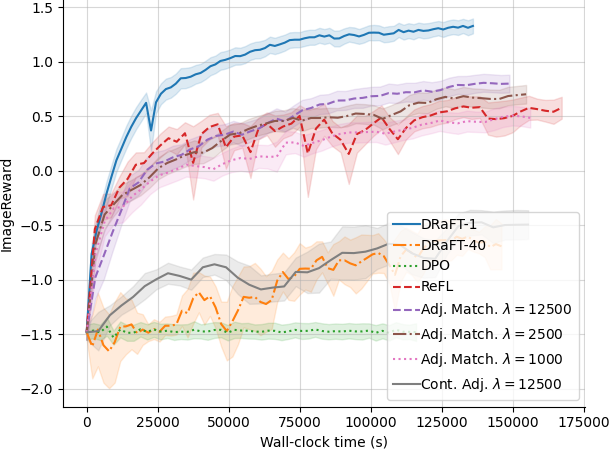
\includegraphics[width=0.46\linewidth]{figs/training_plots/reward_plot.png}
    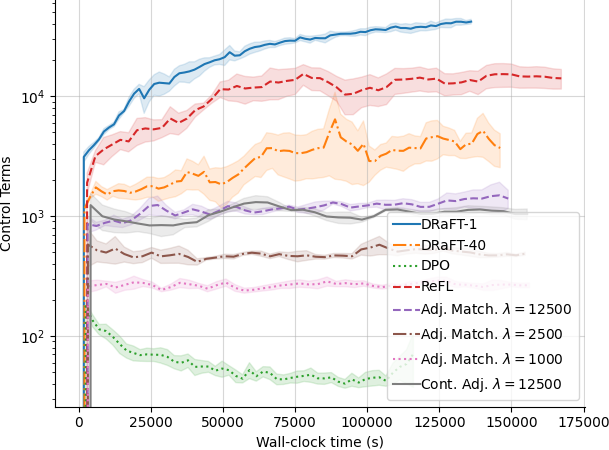
\includegraphics[width=0.46\linewidth]{figs/training_plots/control_term_plot.png}
    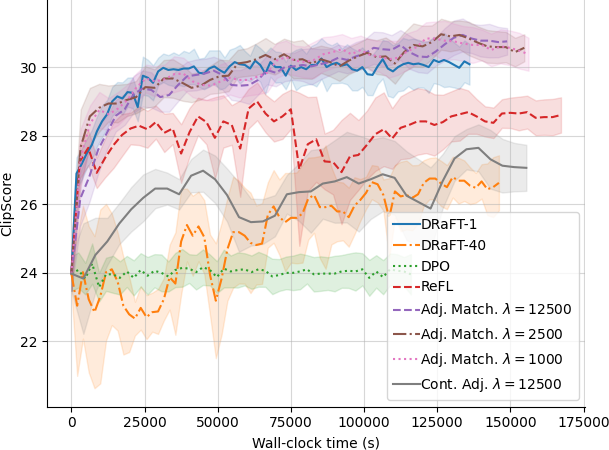
\includegraphics[width=0.46\linewidth]{figs/training_plots/clipscore_plot.png}
    \caption{Average values of ImageReward (reward function), control cost ($\int_0^t \frac{1}{2} \|u(X^u_t,t)\|^2 \, \mathrm{d}t$), and ClipScore vs. wall-clock time for Adjoint Matching and our baselines. Lines show averages over three fine-tuning runs, evaluating on separate test datasets of size 200. Confidence intervals show standard errors of estimates.}
    \label{fig:training_figures}
\end{figure}

\begin{table}[h!]
\centering
{\small
\begin{tabular}{lcccccc}
    \toprule
    Fine-tuning & Fine-tuning & Sampling & \multirow{2}{*}{ImageReward$\, \uparrow$} & ClipScore & PickScore & Total time (s) /
    \\
    loss & $\sigma(t)$ & $\sigma(t)$ &  & diversity$\, \uparrow$ & diversity$\, \uparrow$ & \# iterations \\
    \midrule
    None & \multirow{2}{*}{N/A} & $\sqrt{2 \eta_t}$ & $-$1.384{\tiny$\pm$0.040} & 28.07{\tiny$\pm$1.40} & 1.63{\tiny$\pm$0.08} & \multirow{2}{*}{N/A} 
    \\
    ($\mathrm{CFG}=1.0$)                    &                     & 0                 & $-$0.920{\tiny$\pm$0.042} & 30.29{\tiny$\pm$1.53} & 1.82{\tiny$\pm$0.09} \\
    \midrule
    \multirow{2}{*}{DRaFT-1}           & $\sqrt{2 \eta_t}$ & $\sqrt{2 \eta_t}$ & 1.357{\tiny$\pm$0.039} & 16.86{\tiny$\pm$0.98} & 1.21{\tiny$\pm$0.07} 
    & 140k{\tiny$\pm$5.9k}
    \\
                                       & 0                 & 0                 & 1.251{\tiny$\pm$0.040} & 16.76{\tiny$\pm$1.06} & 1.27{\tiny$\pm$0.07} 
    & / 4000 
    \\
    \addlinespace
    \multirow{2}{*}{DRaFT-40}          & $\sqrt{2 \eta_t}$ & $\sqrt{2 \eta_t}$ & $-$0.560{\tiny$\pm$0.138} & 24.07{\tiny$\pm$1.37} & 1.64{\tiny$\pm$0.12} 
    & 148k{\tiny$\pm$4.2k} 
    \\
                                       & 0                 & 0                 & 0.424{\tiny$\pm$0.042} & 20.99{\tiny$\pm$1.54} & 1.67{\tiny$\pm$0.08} 
    & / 1500 
    \\
    \addlinespace
    \multirow{2}{*}{DPO}          & $\sqrt{2 \eta_t}$ & $\sqrt{2 \eta_t}$ & $-$1.386{\tiny$\pm$0.033} & 27.80{\tiny$\pm$1.40} & 1.62{\tiny$\pm$0.08} 
    & 118k{\tiny$\pm$0.6k} 
    \\
                                       & 0                 & 0                 & $-$0.957{\tiny$\pm$0.040} & 29.81{\tiny$\pm$1.43} & 1.68{\tiny$\pm$0.10} 
    & / 1000
    \\
    \addlinespace
    \multirow{2}{*}{ReFL}              & $\sqrt{2 \eta_t}$ & $\sqrt{2 \eta_t}$ & 0.687{\tiny$\pm$0.085} & 19.49{\tiny$\pm$1.76} & 1.22{\tiny$\pm$0.08} 
    & 173k{\tiny$\pm$10.9k}
    \\
                                       & 0                 & 0                 & 0.709{\tiny$\pm$0.080} & 18.39{\tiny$\pm$1.11} & 1.31{\tiny$\pm$0.10} 
    & / 6000 
    \\
    \midrule % \addlinespace
    Cont. Adjoint & \multirow{2}{*}{$\sqrt{2 \eta_t}$} & $\sqrt{2 \eta_t}$ & $-$0.448{\tiny$\pm$0.135} & 26.97{\tiny$\pm$1.37} & 1.82{\tiny$\pm$0.09} 
    & 153k{\tiny$\pm$0.9k}
    \\
    $\lambda = 12500$                     &                                    & 0                 & $-$0.249{\tiny$\pm$0.116} & 26.25{\tiny$\pm$1.30} & 1.90{\tiny$\pm$0.10} 
    & / 750  
    \\
    \addlinespace
    Disc. Adjoint & \multirow{2}{*}{$\sqrt{2 \eta_t}$} & $\sqrt{2 \eta_t}$ & $-$0.557{\tiny$\pm$0.113} & 30.40{\tiny$\pm$2.39} & 1.91{\tiny$\pm$0.09} 
    & 152k{\tiny$\pm$1.5k}
    \\
    $\lambda = 12500$                    &                                    & 0                 & $-$0.552{\tiny$\pm$0.041} & 28.37{\tiny$\pm$2.26} & 1.97{\tiny$\pm$0.09} 
    & / 1000 
    \\
    \midrule % \addlinespace
    Adj.-Matching  & \multirow{2}{*}{$\sqrt{2 \eta_t}$} & $\sqrt{2 \eta_t}$ & 0.550{\tiny$\pm$0.043} & 23.00{\tiny$\pm$1.27} & 1.65{\tiny$\pm$0.08} 
    &  
    \\
    $\lambda = 1000$                     &                                    & 0                 & 0.454{\tiny$\pm$0.055} & 22.76{\tiny$\pm$1.40} & 1.73{\tiny$\pm$0.09} 
    % &  
    \\
    \addlinespace
    Adj.-Matching & \multirow{2}{*}{$\sqrt{2 \eta_t}$} & $\sqrt{2 \eta_t}$ & 0.755{\tiny$\pm$0.040} & 21.33{\tiny$\pm$1.71} & 1.55{\tiny$\pm$0.08} 
    & 156k{\tiny$\pm$1.9k}
    \\
    $\lambda = 2500$                     &                                    & 0                 & 0.671{\tiny$\pm$0.047} & 21.42{\tiny$\pm$1.54} & 1.64{\tiny$\pm$0.08}
    & / 1000 
    \\
    \addlinespace
    Adj.-Matching  & \multirow{2}{*}{$\sqrt{2 \eta_t}$} & $\sqrt{2 \eta_t}$ & 0.882{\tiny$\pm$0.058} & 20.49{\tiny$\pm$1.48} & 1.50{\tiny$\pm$0.09} 
    & 
    \\
    $\lambda = 12500$                    &                                    & 0                 & 0.778{\tiny$\pm$0.050} & 20.34{\tiny$\pm$1.49} & 1.57{\tiny$\pm$0.09}
    &  
    \\
    \bottomrule
\end{tabular}
}
\caption{Metrics for various fine-tuning methods for text-to-image generation. The second and third columns show the noise schedules $\sigma(t)$ used for fine-tuning and for inference: $\sigma(t) = \sqrt{2\eta_t}$ corresponds to Memoryless Flow Matching, %\eqref{eq:memoryless_FM_sde}, 
and $\sigma(t) = 0$ to the Flow Matching ODE \eqref{eq:FM_ode}. Confidence intervals show standard errors of estimates; computed over 3 runs of the fine-tuning algorithm on separate fine-tuning prompt datasets of size 40000 each. Test prompt sets are of size 1000, and also different for each run.}
\label{table:metrics_multiprompt_diversity}
\end{table}

\begin{table}[h!]
\centering
{\footnotesize
\begin{tabular}{lcccccccc}
    \toprule
    Fine-tun. & Fine-tun. & Generat. & \multirow{2}{*}{ImageReward$\, \uparrow$} & \multirow{2}{*}{ClipScore$\, \uparrow$} & \multirow{2}{*}{PickScore$\, \uparrow$} & \multirow{2}{*}{HPS v2$\, \uparrow$} & DreamSim & Runtime/ \\
    loss & $\sigma(t)$ & $\sigma(t)$ &  & &  &  & diversity$\, \uparrow$ & $\#$iter. \\
    % \midrule
    % \multirow{2}{*}{None (Base)} & \multirow{2}{*}{N/A} & $\sqrt{2 \eta_t}$ & $-\! \pm \!-$ & $-\! \pm \!-$ & $-\! \pm \!-$ & $-\! \pm \!-$ & \multirow{2}{*}{N/A} \\
    %                              &                     & 0                 & $-\! \pm \!-$ & $-\! \pm \!-$ & $-\! \pm \!-$ & $-\! \pm \!-$ &  \\
    \midrule % \addlinespace
    \multirow{2}{*}{ReFL}              & $\sqrt{2 \eta_t}$ & $\sqrt{2 \eta_t}$ & 0.459{\tiny$\pm$0.096} & 28.46{\tiny$\pm$0.25} & 18.77{\tiny$\pm$0.09} & 22.54{\tiny$\pm$0.17} & 37.51{\tiny$\pm$3.50} & 43k{\tiny$\pm$2.7k} \\
                                       & 0                 & 0                 & 0.330{\tiny$\pm$0.114} & 29.63{\tiny$\pm$0.61} & 19.08{\tiny$\pm$0.18} & 22.46{\tiny$\pm$0.77} & 39.51{\tiny$\pm$1.30} & / 1500 \\
    \addlinespace
    \multirow{2}{*}{DRaFT-1}           & $\sqrt{2 \eta_t}$ & $\sqrt{2 \eta_t}$ & 0.913{\tiny$\pm$0.068} & 29.80{\tiny$\pm$0.22} & 19.16{\tiny$\pm$0.06} & 23.63{\tiny$\pm$0.16} & 35.21{\tiny$\pm$1.93} & 35k{\tiny$\pm$1.5k} \\
                                       & 0                 & 0                 & 0.626{\tiny$\pm$0.195} & 30.48{\tiny$\pm$0.32} & 18.91{\tiny$\pm$0.34} & 21.92{\tiny$\pm$1.63} & 38.52{\tiny$\pm$2.01} & / 1000 \\
    \addlinespace
    \multirow{2}{*}{Draft-40}          & $\sqrt{2 \eta_t}$ & $\sqrt{2 \eta_t}$ & $-$1.427{\tiny$\pm$0.267} & 23.39{\tiny$\pm$1.72} & 17.24{\tiny$\pm$0.45} & 15.72{\tiny$\pm$1.80} & 41.98{\tiny$\pm$2.14} & 49k{\tiny$\pm$1.4k} \\
                                       & 0                 & 0                 & $-$0.097{\tiny$\pm$0.052} & 29.12{\tiny$\pm$0.41} & 18.97{\tiny$\pm$0.14} & 21.93{\tiny$\pm$0.20} & 46.35{\tiny$\pm$1.34} & / 500 \\
    \midrule % \addlinespace
    Adj.-Match.  & \multirow{2}{*}{$\sqrt{2 \eta_t}$} & $\sqrt{2 \eta_t}$ & 0.107{\tiny$\pm$0.046} & 29.37{\tiny$\pm$0.25} & 19.05{\tiny$\pm$0.07} & 22.79{\tiny$\pm$0.20} & 46.38{\tiny$\pm$1.36} &  \\
    $\lambda = 1000$                     &                                    & 0                 & 0.051{\tiny$\pm$0.044} & 30.58{\tiny$\pm$0.17} & 19.31{\tiny$\pm$0.07} & 21.93{\tiny$\pm$0.23} & 48.12{\tiny$\pm$1.56} &  \\
    \addlinespace
    Adj.-Match. & \multirow{2}{*}{$\sqrt{2 \eta_t}$} & $\sqrt{2 \eta_t}$ & 0.199{\tiny$\pm$0.068} & 29.27{\tiny$\pm$0.21} & 19.07{\tiny$\pm$0.10} & 22.98{\tiny$\pm$0.30} & 45.03{\tiny$\pm$1.61} & 39k{\tiny$\pm$0.5k} \\
    $\lambda = 2500$                     &                                    & 0                 & 0.106{\tiny$\pm$0.067} & 30.43{\tiny$\pm$0.24} & 19.32{\tiny$\pm$0.11} & 22.16{\tiny$\pm$0.33} & 47.61{\tiny$\pm$1.49} & / 250 \\
    \addlinespace
    Adj.-Match.  & \multirow{2}{*}{$\sqrt{2 \eta_t}$} & $\sqrt{2 \eta_t}$ & 0.299{\tiny$\pm$0.095} & 29.61{\tiny$\pm$0.37} & 19.26{\tiny$\pm$0.14} & 23.67{\tiny$\pm$0.27} & 43.36{\tiny$\pm$1.93} &  \\
    $\lambda = 12500$                    &                                    & 0                 & 0.224{\tiny$\pm$0.051} & 30.70{\tiny$\pm$0.23} & 19.52{\tiny$\pm$0.11} & 22.93{\tiny$\pm$0.21} & 44.62{\tiny$\pm$1.79} &  \\
    \midrule % \addlinespace
    Cont. Adj. & \multirow{2}{*}{$\sqrt{2 \eta_t}$} & $\sqrt{2 \eta_t}$ & $-$0.910{\tiny$\pm$0.116} & 26.29{\tiny$\pm$0.44} & 18.06{\tiny$\pm$0.16} & 18.86{\tiny$\pm$0.88} & 51.60{\tiny$\pm$1.97} & 51k{\tiny$\pm$0.3k} \\
    $\lambda = 12500$                     &                                    & 0                 & $-$0.681{\tiny$\pm$0.051} & 28.50{\tiny$\pm$0.19} & 18.69{\tiny$\pm$0.11} & 19.90{\tiny$\pm$0.50} & 50.87{\tiny$\pm$1.52} & / 250 \\
    \addlinespace
    Disc. Adj. & \multirow{2}{*}{$\sqrt{2 \eta_t}$} & $\sqrt{2 \eta_t}$ & $-$0.978{\tiny$\pm$0.123} & 26.68{\tiny$\pm$0.76} & 18.51{\tiny$\pm$0.11} & 18.53{\tiny$\pm$0.28} & 55.95{\tiny$\pm$1.70} & 38k{\tiny$\pm$0.4k} \\
    $\lambda = 12500$                    &                                    & 0                 & $-$0.791{\tiny$\pm$0.065} & 28.66{\tiny$\pm$0.33} & 18.51{\tiny$\pm$0.11} & 18.53{\tiny$\pm$0.28} & 54.78{\tiny$\pm$2.00} & / 250 \\
    \bottomrule
\end{tabular}
}
\caption{Additional metrics for various fine-tuning methods for text-to-image generation, which complement the ones in \Cref{tab:evaluation_metrics} (both tables correspond to the same runs). The second and third columns show the noise schedules $\sigma(t)$ used for fine-tuning and for inference: $\sigma(t) = \sqrt{2\eta_t}$ corresponds to Memoryless Flow Matching, 
% \eqref{eq:memoryless_FM_sde}, 
and $\sigma(t) = 0$ to the Flow Matching ODE \eqref{eq:FM_ode}.
}
\label{table:metrics_multiprompt_alternative}
\end{table}

\begin{table}[h!]
\centering
{\footnotesize
\begin{tabular}{lllccccccc}
    \toprule
    \multirow{2}{*}{$w$} & Fine-tuning & $\#$iter. & Fine-tun. & Sampl.  & \multirow{2}{*}{ImageReward$\, \uparrow$} & \multirow{2}{*}{ClipScore$\, \uparrow$} & \multirow{2}{*}{PickScore$\, \uparrow$} & \multirow{2}{*}{HPS v2$\, \uparrow$} & DreamSim \\
     & loss & / $\lambda$ & $\sigma(t)$ & $\sigma(t)$ &  &  &  &  & diversity$\, \uparrow$ \\
    \midrule
    \multirow{2}{*}{0.0} & \multirow{2}{*}{None} &  \multirow{2}{*}{N/A}        & \multirow{2}{*}{N/A}          & $\sqrt{2 \eta_t}$         & $-$1.384{\tiny$\pm$0.040} & 24.15{\tiny$\pm$0.26} & 17.25{\tiny$\pm$0.06} & 16.19{\tiny$\pm$0.17} & 53.60{\tiny$\pm$1.37} \\
     &  &       &                & 0                 & $-$0.920{\tiny$\pm$0.042} & 28.32{\tiny$\pm$0.22} & 18.15{\tiny$\pm$0.07} & 17.89{\tiny$\pm$0.16} & \textbf{56.53{\tiny$\pm$1.52}}       
                                    \\
    \midrule
    \multirow{7}{*}{0.0} & \multirow{7}{*}{DRaFT-1} &  \multirow{2}{*}{1000}       & $\sqrt{2 \eta_t}$ & $\sqrt{2 \eta_t}$ & 0.913{\tiny$\pm$0.068} & 29.80{\tiny$\pm$0.22} & 19.16{\tiny$\pm$0.06} & 23.63{\tiny$\pm$0.16} & 35.21{\tiny$\pm$1.93} \\
    & &  & 0                 & 0                 & 0.626{\tiny$\pm$0.195} & 30.48{\tiny$\pm$0.32} & 18.91{\tiny$\pm$0.34} & 21.92{\tiny$\pm$1.63} & 38.52{\tiny$\pm$2.01} \\
    % \midrule
    \addlinespace
     &  &  \multirow{2}{*}{2000}       & $\sqrt{2 \eta_t}$ & $\sqrt{2 \eta_t}$ & 1.204{\tiny$\pm$0.046} & 29.90{\tiny$\pm$0.43} & 19.29{\tiny$\pm$0.12} & 24.40{\tiny$\pm$0.27} & 28.51{\tiny$\pm$1.68} \\
                                   & &  & 0                 & 0                 & 1.052{\tiny$\pm$0.088} & 30.65{\tiny$\pm$0.24} & 19.27{\tiny$\pm$0.11} & 23.81{\tiny$\pm$0.44} & 32.11{\tiny$\pm$2.37} \\
    % \midrule
    \addlinespace
    & &  \multirow{2}{*}{3000}       & $\sqrt{2 \eta_t}$ & $\sqrt{2 \eta_t}$ & \textbf{1.307{\tiny$\pm$0.041}} & 29.96{\tiny$\pm$0.22} & 19.31{\tiny$\pm$0.06} & 24.42{\tiny$\pm$0.13} & 26.57{\tiny$\pm$1.32} \\
                                   & &  & 0                 & 0                 & 1.173{\tiny$\pm$0.058} & 30.86{\tiny$\pm$0.25} & 19.37{\tiny$\pm$0.06} & 24.17{\tiny$\pm$0.23} & 29.69{\tiny$\pm$1.30}
    \\
    \addlinespace
    & &  \multirow{2}{*}{4000}       & $\sqrt{2 \eta_t}$ & $\sqrt{2 \eta_t}$ & \textbf{1.357{\tiny$\pm$0.039}} & 30.18{\tiny$\pm$0.24} & 19.38{\tiny$\pm$0.08} & 24.61{\tiny$\pm$0.17} & 25.54{\tiny$\pm$0.99} \\
                                   & &  & 0                 & 0                 & 1.251{\tiny$\pm$0.040} & 30.95{\tiny$\pm$0.28} & 19.37{\tiny$\pm$0.06} & 24.37{\tiny$\pm$0.17} & 27.39{\tiny$\pm$1.14}
    \\
    \midrule
    \multirow{7}{*}{0.0} & \multirow{7}{*}{Adj.-Match.} & \multirow{2}{*}{1000} & $\sqrt{2 \eta_t}$ & $\sqrt{2 \eta_t}$  & 0.550{\tiny$\pm$0.043} & 30.36{\tiny$\pm$0.22} & 19.29{\tiny$\pm$0.08} & 24.12{\tiny$\pm$0.17} & 40.89{\tiny$\pm$1.50} \\
     & &  & 0                 & 0                 & 0.454{\tiny$\pm$0.055} &  31.41{\tiny$\pm$0.22} & 19.57{\tiny$\pm$0.09} & 23.29{\tiny$\pm$0.18} & 43.10{\tiny$\pm$1.76} \\
    \addlinespace
    & & \multirow{2}{*}{2500} & $\sqrt{2 \eta_t}$ & $\sqrt{2 \eta_t}$ & 0.755{\tiny$\pm$0.040} & 30.59{\tiny$\pm$0.40} & 19.49{\tiny$\pm$0.10} & 24.85{\tiny$\pm$0.23} & 37.07{\tiny$\pm$1.47} \\
    & &  & 0 & 0 & 0.671{\tiny$\pm$0.047} & 31.64{\tiny$\pm$0.21} & 19.71{\tiny$\pm$0.09} & 24.12{\tiny$\pm$0.27} & 39.88{\tiny$\pm$1.59} \\
    \addlinespace
    & & \multirow{2}{*}{12500} & $\sqrt{2 \eta_t}$ & $\sqrt{2 \eta_t}$ & 0.882{\tiny$\pm$0.058} & 30.62{\tiny$\pm$0.30} & 19.50{\tiny$\pm$0.09} & 24.95{\tiny$\pm$0.28} & 34.50{\tiny$\pm$1.33} \\
    & &  & 0 & 0 & 0.778{\tiny$\pm$0.050} & 31.65{\tiny$\pm$0.19} & 19.76{\tiny$\pm$0.08} & 24.49{\tiny$\pm$0.27} & 37.24{\tiny$\pm$1.57} \\
    \midrule
    \multirow{2}{*}{1.0} & \multirow{2}{*}{None} &  \multirow{2}{*}{N/A}        & \multirow{2}{*}{N/A}          & $\sqrt{2 \eta_t}$         & $-$0.269{\tiny$\pm$0.050} & 30.41{\tiny$\pm$0.22} & 18.74{\tiny$\pm$0.07} & 20.47{\tiny$\pm$0.18} & 43.82{\tiny$\pm$1.24} \\
     &  &       &                & 0                 & $-$0.123{\tiny$\pm$0.041} & 31.83{\tiny$\pm$0.17} & 19.28{\tiny$\pm$0.07} & 20.95{\tiny$\pm$0.16} & 42.59{\tiny$\pm$1.23}                             
                                    \\
    \midrule
    \multirow{6}{*}{1.0} & \multirow{6}{*}{DRaFT-1} &  \multirow{2}{*}{1000}        & $\sqrt{2 \eta_t}$          & $\sqrt{2 \eta_t}$         & 1.123{\tiny$\pm$0.051} & 32.06{\tiny$\pm$0.19} & 19.69{\tiny$\pm$0.06} & 24.56{\tiny$\pm$0.17} & 28.25{\tiny$\pm$1.55} \\
     &  &       & 0                 & 0                 & 0.856{\tiny$\pm$0.167} & 32.32{\tiny$\pm$0.25} & 19.38{\tiny$\pm$0.34} & 22.88{\tiny$\pm$1.54} & 29.98{\tiny$\pm$1.86} \\
    % \midrule
    \addlinespace
     &  &  2000        & 0                 & 0                 & 1.177{\tiny$\pm$0.053} & 32.36{\tiny$\pm$0.18} & 19.67{\tiny$\pm$0.08} & 24.48{\tiny$\pm$0.28} & 25.09{\tiny$\pm$1.82} \\
    % \midrule
    \addlinespace
    & & 3000 & 0                 & 0                 & 1.255{\tiny$\pm$0.038} & 32.36{\tiny$\pm$0.19} & 19.70{\tiny$\pm$0.06} & 24.64{\tiny$\pm$0.17} & 23.24{\tiny$\pm$1.19} \\
    \addlinespace
    & &  4000  & 0 & 0 & \textbf{1.296{\tiny$\pm$0.033}} & 32.30{\tiny$\pm$0.19} & 19.68{\tiny$\pm$0.06} & 24.71{\tiny$\pm$0.14} & 21.54{\tiny$\pm$0.96} \\
    \midrule
    \multirow{5}{*}{1.0} & \multirow{5}{*}{Adj.-Match.} & 1000 & 0                 & 0                 & 0.782{\tiny$\pm$0.044} & 33.05{\tiny$\pm$0.22} & 20.20{\tiny$\pm$0.09} & 24.81{\tiny$\pm$0.18} & 32.67{\tiny$\pm$1.26} \\
    \addlinespace
    & & \multirow{2}{*}{2500} & $\sqrt{2 \eta_t}$ & $\sqrt{2 \eta_t}$ & 1.027{\tiny$\pm$0.038} & 32.85{\tiny$\pm$0.21} & 20.08{\tiny$\pm$0.08} & \textbf{25.88{\tiny$\pm$0.20}} & 29.83{\tiny$\pm$1.00} \\
    & &  & 0 & 0 & 0.910{\tiny$\pm$0.040} & 33.20{\tiny$\pm$0.17} & 20.29{\tiny$\pm$0.09} & 25.39{\tiny$\pm$0.24} & 30.34{\tiny$\pm$1.51} \\
    \addlinespace
    & & 12500 & 0 & 0 & 0.985{\tiny$\pm$0.041} & 33.10{\tiny$\pm$0.18} & 20.28{\tiny$\pm$0.08} & \textbf{25.61{\tiny$\pm$0.27}} & 28.86{\tiny$\pm$1.37} \\
    \midrule
    \multirow{2}{*}{4.0} & \multirow{2}{*}{None} &  \multirow{2}{*}{N/A}        & \multirow{2}{*}{N/A}          & $\sqrt{2 \eta_t}$         & 0.277{\tiny$\pm$0.043} & 32.68{\tiny$\pm$0.18} & 19.50{\tiny$\pm$0.07} & 22.29{\tiny$\pm$0.16} & 35.12{\tiny$\pm$0.92} \\
     &  &       &                & 0                 & 0.209{\tiny$\pm$0.046} & 32.83{\tiny$\pm$0.17} & 19.79{\tiny$\pm$0.07} & 22.30{\tiny$\pm$0.17} & 32.05{\tiny$\pm$1.05}    
                                    \\
    \midrule
    \multirow{6}{*}{4.0} & \multirow{6}{*}{DRaFT-1} &  \multirow{2}{*}{1000}        & $\sqrt{2 \eta_t}$          & $\sqrt{2 \eta_t}$         & 1.062{\tiny$\pm$0.045} & 32.29{\tiny$\pm$0.16} & 19.48{\tiny$\pm$0.06} & 23.67{\tiny$\pm$0.13} & 25.03{\tiny$\pm$1.32} \\
     &  &       & 0                 & 0                 & 0.604{\tiny$\pm$0.395} & 31.80{\tiny$\pm$0.86} & 19.09{\tiny$\pm$0.53} & 21.69{\tiny$\pm$2.10} & 25.92{\tiny$\pm$2.57} \\
    % \midrule
    \addlinespace
     &  &  2000        & 0                 & 0                 & 1.112{\tiny$\pm$0.046} & 32.29{\tiny$\pm$0.20} & 19.34{\tiny$\pm$0.11} & 23.31{\tiny$\pm$0.22} & 21.02{\tiny$\pm$1.67} \\
    % \midrule
    \addlinespace
    & & 3000 & 0                 & 0                 & 1.151{\tiny$\pm$0.036} & 32.31{\tiny$\pm$0.21} & 19.36{\tiny$\pm$0.06} & 23.29{\tiny$\pm$0.14} & 19.53{\tiny$\pm$1.24} \\
    \addlinespace
    & &  4000  & 0 & 0 & 1.172{\tiny$\pm$0.040} & 32.20{\tiny$\pm$0.22} & 19.30{\tiny$\pm$0.07} & 23.20{\tiny$\pm$0.15} & 18.45{\tiny$\pm$1.06} \\
    \midrule
    \multirow{5}{*}{4.0} & \multirow{5}{*}{Adj.-Match.} & 1000 & 0                 & 0                 & 0.852{\tiny$\pm$0.046} & \textbf{33.50{\tiny$\pm$0.22}} & 20.31{\tiny$\pm$0.08} & 24.97{\tiny$\pm$0.19} & 25.83{\tiny$\pm$0.82} \\
    \addlinespace
    & & \multirow{2}{*}{2500} & $\sqrt{2 \eta_t}$ & $\sqrt{2 \eta_t}$ & 1.052{\tiny$\pm$0.039} & \textbf{33.51}{\tiny$\pm$0.19} & 20.15{\tiny$\pm$0.07} & \textbf{25.56{\tiny$\pm$0.18}} & 26.21{\tiny$\pm$0.73} \\
    & &  & 0 & 0 & 0.942{\tiny$\pm$0.042} & \textbf{33.61}{\tiny$\pm$0.19} & \textbf{20.35}{\tiny$\pm$0.08} & 25.34{\tiny$\pm$0.21} & 24.30{\tiny$\pm$0.86} \\
    \addlinespace
    & & 12500 & 0 & 0 & 1.007{\tiny$\pm$0.052} & \textbf{33.48{\tiny$\pm$0.20}} & 20.29{\tiny$\pm$0.08} & \textbf{25.50{\tiny$\pm$0.29}} & 23.48{\tiny$\pm$0.81} \\
    \bottomrule
\end{tabular}
}
\caption{ 
Evaluation metrics when using classifier-free guidance (CFG; \citet{ho2022classifier}).
}
\end{table}

\begin{table}[h!]
\centering
{\footnotesize
\begin{tabular}{llccccccc}
    \toprule
    LR / & Fine-tuning & Fine-tun. & Generat. & \multirow{2}{*}{ImageReward$\, \uparrow$} & \multirow{2}{*}{ClipScore$\, \uparrow$} & \multirow{2}{*}{PickScore$\, \uparrow$} & \multirow{2}{*}{HPS v2$\, \uparrow$} & DreamSim \\
    Adam $\beta_1$ & loss & $\sigma(t)$ & $\sigma(t)$ & & &  &  & diversity$\, \uparrow$ \\
    \midrule
    \num{3e-5} & DRaFT-1          & $\sqrt{2 \eta_t}$ & $\sqrt{2 \eta_t}$ & 1.467{\tiny$\pm$0.029} & 30.28{\tiny$\pm$0.56} & 19.37{\tiny$\pm$0.09} & 24.70{\tiny$\pm$0.15} & 21.20{\tiny$\pm$0.93} \\
               % &  &  & $\num{3e-5} / 0.97$ & $- \pm -$ & $- \pm -$ & $- \pm -$ & $- \pm -$ \\
    \addlinespace
    / \num{0.97} & Adj.-Match.  & \multirow{2}{*}{$\sqrt{2 \eta_t}$} & \multirow{2}{*}{$\sqrt{2 \eta_t}$} & \multirow{2}{*}{1.130{\tiny$\pm$0.034}} & \multirow{2}{*}{31.01{\tiny$\pm$0.27}} & \multirow{2}{*}{19.60{\tiny$\pm$0.08}} & \multirow{2}{*}{25.01{\tiny$\pm$0.25}} & \multirow{2}{*}{26.73{\tiny$\pm$0.88}} \\
    & $\lambda = 12500$                     &                                    &                 &  &  &  &  &  \\
    \midrule
    \num{2e-5} & Disc. Adj.  & $\sqrt{2 \eta_t}$ & $\sqrt{2 \eta_t}$ & $-$1.186{\tiny$\pm$0.553} & 21.95{\tiny$\pm$4.29} & 16.94{\tiny$\pm$0.95} & 12.34{\tiny$\pm$4.40} & 28.33{\tiny$\pm$10.26} \\
     / \num{0.95} & $\lambda = 12500$                     &  0                                  &  0               & $-$0.961{\tiny$\pm$0.653} & 24.07{\tiny$\pm$4.71} & 17.86{\tiny$\pm$1.17} & 15.93{\tiny$\pm$5.80} & 33.62{\tiny$\pm$7.80} \\
    \bottomrule
\end{tabular}
}
\caption{Metrics for alternative optimization hyperparameters (learning rate and Adam $\beta_1$). 
% learning rate $=\num{3e-5}$ and Adam $\beta_1=$ 0.97, in contrast to the values $\num{2e-5}$ and 0.95 used elsewhere.
}
\label{table:alternative_hyperparameters}
\end{table}

\begin{table}[h!]
\centering
{\footnotesize
\begin{tabular}{lccccccc}
    \toprule
    Fine-tuning & Fine-tuning & Generative & \multirow{2}{*}{ImageReward$\, \uparrow$} & \multirow{2}{*}{ClipScore$\, \uparrow$} & \multirow{2}{*}{PickScore$\, \uparrow$} & \multirow{2}{*}{HPS v2$\, \uparrow$} & DreamSim \\
    loss & $\sigma(t)$ & $\sigma(t)$ & & &  &  & diversity$\, \uparrow$ \\
    \midrule
    Adj.-Matching  & \multirow{2}{*}{1} & 1 & 0.009{\tiny$\pm$0.077} & 29.18{\tiny$\pm$0.51} & 18.66{\tiny$\pm$0.09} & 20.75{\tiny$\pm$0.32} & 41.33{\tiny$\pm$1.24} \\
    $\lambda = 12500$                     &                                    &  0               & 0.454{\tiny$\pm$0.055} & 31.41{\tiny$\pm$0.22} & 19.57{\tiny$\pm$0.09} & 23.29{\tiny$\pm$0.18} & 43.10{\tiny$\pm$1.76} \\
    \addlinespace
    Adj.-Matching  & \multirow{2}{*}{$\sqrt{2 \eta_t}$} & $\sqrt{2 \eta_t}$ & 0.882{\tiny$\pm$0.058} & 30.62{\tiny$\pm$0.30} & 19.50{\tiny$\pm$0.09} & 24.95{\tiny$\pm$0.28} & 34.50{\tiny$\pm$1.33}  \\
    $\lambda = 12500$                    &                                    & 0                 & 0.778{\tiny$\pm$0.050} & 31.65{\tiny$\pm$0.19} & 19.76{\tiny$\pm$0.08} & 24.49{\tiny$\pm$0.27} & 37.24{\tiny$\pm$1.57}  \\
    \bottomrule
\end{tabular}
}
\caption{Comparison with an alternative fine-tuning noise schedule $\sigma(t)=1$. We see that the initial value function bias (\Cref{sec:value_function_bias_problem}) results in the model not having a high reward function (ImageReward is the reward function used for fine-tuning). Its performance on other metrics are also lower than when fine-tuning with the memoryless noise schedule, except for diversity.}
\label{table:alternative_noise_schedule}
\end{table}

\begin{table}[h!]
\centering
{\footnotesize
\begin{tabular}{llccccccc}
    \toprule
    $\#$sampl. & Fine-tuning & Fine-tun. & Sampl. & \multirow{2}{*}{ImageReward$\, \uparrow$} & \multirow{2}{*}{ClipScore$\, \uparrow$} & \multirow{2}{*}{PickScore$\, \uparrow$} & \multirow{2}{*}{HPS v2$\, \uparrow$} & DreamSim \\
    timesteps & loss & $\sigma(t)$ & $\sigma(t)$ &  &  &  &  & diversity$\, \uparrow$ \\
    \midrule
    \multirow{6}{*}{$10$} & \multirow{2}{*}{None (Base)} & \multirow{2}{*}{N/A} & $\sqrt{2 \eta_t}$ & $-$2.279{\tiny$\pm$0.001} & 13.99{\tiny$\pm$0.12} & 14.98{\tiny$\pm$0.05} & 7.37{\tiny$\pm$0.10} & 5.07{\tiny$\pm$0.13} \\
                            &     &                     & 0                 & $-$1.386{\tiny$\pm$0.040} & 26.26{\tiny$\pm$0.24} & 17.64{\tiny$\pm$0.07} & 14.92{\tiny$\pm$0.17} & 51.26{\tiny$\pm$1.38} \\
    \addlinespace
     & \multirow{2}{*}{DRaFT-1}           & $\sqrt{2 \eta_t}$ & $\sqrt{2 \eta_t}$ & 1.033{\tiny$\pm$0.051} & 25.98{\tiny$\pm$0.25} & 18.28{\tiny$\pm$0.07} & 22.08{\tiny$\pm$0.18} & 14.47{\tiny$\pm$0.67} \\
                                    &   & 0                 & 0                 & 1.236{\tiny$\pm$0.038} & 31.54{\tiny$\pm$0.27} & 19.53{\tiny$\pm$0.07} & 24.47{\tiny$\pm$0.19} & 24.78{\tiny$\pm$0.88} \\
    \addlinespace
     & Adj.-Match.  & \multirow{2}{*}{$\sqrt{2 \eta_t}$} & $\sqrt{2 \eta_t}$ & $-$2.104{\tiny$\pm$0.074} & 17.12{\tiny$\pm$0.56} & 15.76{\tiny$\pm$0.20} & 11.48{\tiny$\pm$1.03} & 9.88{\tiny$\pm$0.81} \\
     & $\lambda = 12500$                     &                                    & 0                 & 0.607{\tiny$\pm$0.055} & 31.36{\tiny$\pm$0.20} & 19.56{\tiny$\pm$0.08} & 23.23{\tiny$\pm$0.28} & 33.75{\tiny$\pm$1.48} \\
    \midrule
    \multirow{6}{*}{$20$} & \multirow{2}{*}{None (Base)} & \multirow{2}{*}{N/A} & $\sqrt{2 \eta_t}$ & $-$2.275{\tiny$\pm$0.002} & 14.58{\tiny$\pm$0.13} & 15.07{\tiny$\pm$0.05} & 7.47{\tiny$\pm$0.10} & 11.27{\tiny$\pm$0.33} \\
                         &        &                     & 0                 &  $-$1.017{\tiny$\pm$0.055} & 27.92{\tiny$\pm$0.19} & 18.01{\tiny$\pm$0.07} & 17.17{\tiny$\pm$0.15} & 54.69{\tiny$\pm$1.45} \\
    \addlinespace
     & \multirow{2}{*}{DRaFT-1}           & $\sqrt{2 \eta_t}$ & $\sqrt{2 \eta_t}$ & \textbf{1.301{\tiny$\pm$0.039}} & 27.09{\tiny$\pm$0.24} & 18.93{\tiny$\pm$0.07} & 23.78{\tiny$\pm$0.20} & 21.05{\tiny$\pm$1.12} \\
                                    &   & 0                 & 0                 & 1.255{\tiny$\pm$0.038} & 31.14{\tiny$\pm$0.25} & 19.43{\tiny$\pm$0.06} & 24.52{\tiny$\pm$0.16} & 26.15{\tiny$\pm$1.11} \\
    \addlinespace
     & Adj.-Match.  & \multirow{2}{*}{$\sqrt{2 \eta_t}$} & $\sqrt{2 \eta_t}$ & $-$0.032{\tiny$\pm$0.072} & 25.07{\tiny$\pm$0.27} & 18.01{\tiny$\pm$0.07} & 20.75{\tiny$\pm$0.23} & 29.06{\tiny$\pm$2.34} \\
     & $\lambda = 12500$                     &                                    & 0                 & 0.768{\tiny$\pm$0.048} & \textbf{31.70{\tiny$\pm$0.17}} & \textbf{19.73{\tiny$\pm$0.08}} & 24.30{\tiny$\pm$0.26} & 35.90{\tiny$\pm$1.52} \\
     \midrule
    \multirow{6}{*}{$40$} & \multirow{2}{*}{None (Base)} & \multirow{2}{*}{N/A} & $\sqrt{2 \eta_t}$ & $-$1.384{\tiny$\pm$0.040} & 24.15{\tiny$\pm$0.26} & 17.25{\tiny$\pm$0.06} & 16.19{\tiny$\pm$0.17} & 53.60{\tiny$\pm$1.37} \\
                         &        &                     & 0                 & $-$0.920{\tiny$\pm$0.042} & 28.32{\tiny$\pm$0.22} & 18.15{\tiny$\pm$0.07} & 17.89{\tiny$\pm$0.16} & \textbf{56.53{\tiny$\pm$1.52}} \\
    \addlinespace
     & \multirow{2}{*}{DRaFT-1}           & $\sqrt{2 \eta_t}$ & $\sqrt{2 \eta_t}$ & \textbf{1.357{\tiny$\pm$0.039}} & 30.18{\tiny$\pm$0.24} & 19.38{\tiny$\pm$0.08} & 24.61{\tiny$\pm$0.17} & 25.54{\tiny$\pm$0.99} \\
                                    &   & 0                 & 0                 & 1.251{\tiny$\pm$0.040} & 30.95{\tiny$\pm$0.28} & 19.37{\tiny$\pm$0.06} & 24.37{\tiny$\pm$0.17} & 27.39{\tiny$\pm$1.14} \\
    \addlinespace
     & Adj.-Match.  & \multirow{2}{*}{$\sqrt{2 \eta_t}$} & $\sqrt{2 \eta_t}$ & 0.882{\tiny$\pm$0.058} & 30.62{\tiny$\pm$0.30} & 19.50{\tiny$\pm$0.09} & \textbf{24.95{\tiny$\pm$0.28}} & 34.50{\tiny$\pm$1.33} \\
     & $\lambda = 12500$                     &                                    & 0                 & 0.778{\tiny$\pm$0.050} & \textbf{31.65{\tiny$\pm$0.19}} & \textbf{19.76{\tiny$\pm$0.08}} & 24.49{\tiny$\pm$0.27} & 37.24{\tiny$\pm$1.57} \\
    \midrule
    \multirow{6}{*}{$100$} & \multirow{2}{*}{None (Base)} & \multirow{2}{*}{N/A} & $\sqrt{2 \eta_t}$ & $-$0.881{\tiny$\pm$0.041} & 27.83{\tiny$\pm$0.19} & 18.10{\tiny$\pm$0.07} & 18.43{\tiny$\pm$0.17} & \textbf{57.21{\tiny$\pm$1.50}} \\
                         &        &                     & 0                 & $-$0.881{\tiny$\pm$0.036} & 28.65{\tiny$\pm$0.18} & 18.22{\tiny$\pm$0.06} & 18.20{\tiny$\pm$0.17} & \textbf{57.73{\tiny$\pm$1.68}} \\
    \addlinespace
     & \multirow{2}{*}{DRaFT-1}           & $\sqrt{2 \eta_t}$ & $\sqrt{2 \eta_t}$ & \textbf{1.343{\tiny$\pm$0.040}} & 30.64{\tiny$\pm$0.20} & 19.38{\tiny$\pm$0.08} & 24.37{\tiny$\pm$0.17} & 25.51{\tiny$\pm$1.10} \\
                                    &   & 0                 & 0                 & 1.239{\tiny$\pm$0.037} & 30.74{\tiny$\pm$0.28} & 19.33{\tiny$\pm$0.06} & 24.24{\tiny$\pm$0.17} & 28.70{\tiny$\pm$1.11} \\
    \addlinespace
     & Adj.-Match.  & \multirow{2}{*}{$\sqrt{2 \eta_t}$} & $\sqrt{2 \eta_t}$ & 0.892{\tiny$\pm$0.044} & 31.23{\tiny$\pm$0.23} & \textbf{19.65{\tiny$\pm$0.08}} & \textbf{24.92{\tiny$\pm$0.23}} & 35.13{\tiny$\pm$1.40} \\
     & $\lambda = 12500$                     &                                    & 0                 & 0.779{\tiny$\pm$0.048} & \textbf{31.64{\tiny$\pm$0.17}} & \textbf{19.76{\tiny$\pm$0.08}} & 24.57{\tiny$\pm$0.25} & 38.26{\tiny$\pm$1.65} \\
    \midrule
    \multirow{6}{*}{$200$} & \multirow{2}{*}{None (Base)} & \multirow{2}{*}{N/A} & $\sqrt{2 \eta_t}$ & $-$0.848{\tiny$\pm$0.048} & 28.37{\tiny$\pm$0.21} & 18.27{\tiny$\pm$0.08} & 18.56{\tiny$\pm$0.19} & \textbf{58.00{\tiny$\pm$1.58}} \\
                         &        &                     & 0                 & $-$0.871{\tiny$\pm$0.036} & 28.50{\tiny$\pm$0.18} & 18.23{\tiny$\pm$0.06} & 18.25{\tiny$\pm$0.14} & \textbf{57.84{\tiny$\pm$1.60}} \\
    \addlinespace
     & \multirow{2}{*}{DRaFT-1}           & $\sqrt{2 \eta_t}$ & $\sqrt{2 \eta_t}$ & \textbf{1.331{\tiny$\pm$0.044}} & 30.69{\tiny$\pm$0.23} & 19.36{\tiny$\pm$0.07} & 24.21{\tiny$\pm$0.17} & 26.41{\tiny$\pm$1.18} \\
                                    &   & 0                 & 0                 & 1.222{\tiny$\pm$0.042} & 30.77{\tiny$\pm$0.27} & 19.32{\tiny$\pm$0.06} & 24.18{\tiny$\pm$0.16} & 29.09{\tiny$\pm$1.07} \\
    \addlinespace
     & Adj.-Match.  & \multirow{2}{*}{$\sqrt{2 \eta_t}$} & $\sqrt{2 \eta_t}$ & 0.869{\tiny$\pm$0.062} & 31.33{\tiny$\pm$0.21} & \textbf{19.68{\tiny$\pm$0.09}} & \textbf{24.81{\tiny$\pm$0.30}} & 35.90{\tiny$\pm$1.55} \\
     & $\lambda = 12500$                     &                                    & 0                 & 0.766{\tiny$\pm$0.050} & \textbf{31.61{\tiny$\pm$0.16}} & \textbf{19.75{\tiny$\pm$0.08}} & 24.52{\tiny$\pm$0.24} & 38.60{\tiny$\pm$1.38} \\
    \bottomrule
\end{tabular}
}
\caption{Performance metrics for different number of sampling steps. Only the number of sampling steps is ablated; the fine-tuned models used in all cases are the ones fine-tuned using 40 steps.
}
\label{table:metrics_multiprompt_sampling_steps}
\end{table}

% \begin{table}[h!]
% \centering
% {\footnotesize
% \begin{tabular}{lcccccccc}
%     \toprule
%     Fine-tun. & Fine-tun. & Generat. & \multirow{2}{*}{ImageReward$\, \uparrow$} & \multirow{2}{*}{ClipScore$\, \uparrow$} & \multirow{2}{*}{PickScore$\, \uparrow$} & \multirow{2}{*}{HPS v2$\, \uparrow$} & DreamSim & Runtime/ \\
%     loss & $\sigma(t)$ & $\sigma(t)$ &  & &  &  & diversity$\, \uparrow$ & $\#$iter. \\
%     % \midrule
%     % \multirow{2}{*}{None (Base)} & \multirow{2}{*}{N/A} & $\sqrt{2 \eta_t}$ & $-\! \pm \!-$ & $-\! \pm \!-$ & $-\! \pm \!-$ & $-\! \pm \!-$ & \multirow{2}{*}{N/A} \\
%     %                              &                     & 0                 & $-\! \pm \!-$ & $-\! \pm \!-$ & $-\! \pm \!-$ & $-\! \pm \!-$ &  \\
%     \midrule % \addlinespace
%     \multirow{2}{*}{ReFL}              & $\sqrt{2 \eta_t}$ & $\sqrt{2 \eta_t}$ & 0.459{\tiny$\pm$0.096} & 28.46{\tiny$\pm$0.25} & 18.77{\tiny$\pm$0.09} & 22.54{\tiny$\pm$0.17} & 37.51{\tiny$\pm$3.50} & 43k{\tiny$\pm$2.7k} \\
%                                        & 0                 & 0                 & 0.330{\tiny$\pm$0.114} & 29.63{\tiny$\pm$0.61} & 19.08{\tiny$\pm$0.18} & 22.46{\tiny$\pm$0.77} & 39.51{\tiny$\pm$1.30} & / 1500 \\
%     \addlinespace
%     \multirow{2}{*}{DRaFT-1}           & $\sqrt{2 \eta_t}$ & $\sqrt{2 \eta_t}$ & 0.913{\tiny$\pm$0.068} & 29.80{\tiny$\pm$0.22} & 19.16{\tiny$\pm$0.06} & 23.63{\tiny$\pm$0.16} & 35.21{\tiny$\pm$1.93} & 35k{\tiny$\pm$1.5k} \\
%                                        & 0                 & 0                 & 0.626{\tiny$\pm$0.195} & 30.48{\tiny$\pm$0.32} & 18.91{\tiny$\pm$0.34} & 21.92{\tiny$\pm$1.63} & 38.52{\tiny$\pm$2.01} & / 1000 \\
%     \addlinespace
%     \multirow{2}{*}{Draft-40}          & $\sqrt{2 \eta_t}$ & $\sqrt{2 \eta_t}$ & $-$1.427{\tiny$\pm$0.267} & 23.39{\tiny$\pm$1.72} & 17.24{\tiny$\pm$0.45} & 15.72{\tiny$\pm$1.80} & 41.98{\tiny$\pm$2.14} & 49k{\tiny$\pm$1.4k} \\
%                                        & 0                 & 0                 & $-$0.097{\tiny$\pm$0.052} & 29.12{\tiny$\pm$0.41} & 18.97{\tiny$\pm$0.14} & 21.93{\tiny$\pm$0.20} & 46.35{\tiny$\pm$1.34} & / 500 \\
%     \midrule % \addlinespace
%     Adj.-Match.  & \multirow{2}{*}{$\sqrt{2 \eta_t}$} & $\sqrt{2 \eta_t}$ & 0.107{\tiny$\pm$0.046} & 29.37{\tiny$\pm$0.25} & 19.05{\tiny$\pm$0.07} & 22.79{\tiny$\pm$0.20} & 46.38{\tiny$\pm$1.36} &  \\
%     $\lambda = 1000$                     &                                    & 0                 & 0.051{\tiny$\pm$0.044} & 30.58{\tiny$\pm$0.17} & 19.31{\tiny$\pm$0.07} & 21.93{\tiny$\pm$0.23} & 48.12{\tiny$\pm$1.56} &  \\
%     \addlinespace
%     Adj.-Match. & \multirow{2}{*}{$\sqrt{2 \eta_t}$} & $\sqrt{2 \eta_t}$ & 0.199{\tiny$\pm$0.068} & 29.27{\tiny$\pm$0.21} & 19.07{\tiny$\pm$0.10} & 22.98{\tiny$\pm$0.30} & 45.03{\tiny$\pm$1.61} & 39k{\tiny$\pm$0.5k} \\
%     $\lambda = 2500$                     &                                    & 0                 & 0.106{\tiny$\pm$0.067} & 30.43{\tiny$\pm$0.24} & 19.32{\tiny$\pm$0.11} & 22.16{\tiny$\pm$0.33} & 47.61{\tiny$\pm$1.49} & / 250 \\
%     \addlinespace
%     Adj.-Match.  & \multirow{2}{*}{$\sqrt{2 \eta_t}$} & $\sqrt{2 \eta_t}$ & 0.299{\tiny$\pm$0.095} & 29.61{\tiny$\pm$0.37} & 19.26{\tiny$\pm$0.14} & 23.67{\tiny$\pm$0.27} & 43.36{\tiny$\pm$1.93} &  \\
%     $\lambda = 12500$                    &                                    & 0                 & 0.224{\tiny$\pm$0.051} & 30.70{\tiny$\pm$0.23} & 19.52{\tiny$\pm$0.11} & 22.93{\tiny$\pm$0.21} & 44.62{\tiny$\pm$1.79} &  \\
%     \midrule % \addlinespace
%     Cont. Adj. & \multirow{2}{*}{$\sqrt{2 \eta_t}$} & $\sqrt{2 \eta_t}$ & $-$0.910{\tiny$\pm$0.116} & 26.29{\tiny$\pm$0.44} & 18.06{\tiny$\pm$0.16} & 18.86{\tiny$\pm$0.88} & 51.60{\tiny$\pm$1.97} & 51k{\tiny$\pm$0.3k} \\
%     $\lambda = 12500$                     &                                    & 0                 & $-$0.681{\tiny$\pm$0.051} & 28.50{\tiny$\pm$0.19} & 18.69{\tiny$\pm$0.11} & 19.90{\tiny$\pm$0.50} & 50.87{\tiny$\pm$1.52} & / 250 \\
%     \addlinespace
%     Disc. Adj. & \multirow{2}{*}{$\sqrt{2 \eta_t}$} & $\sqrt{2 \eta_t}$ & $-$0.978{\tiny$\pm$0.123} & 26.68{\tiny$\pm$0.76} & 18.51{\tiny$\pm$0.11} & 18.53{\tiny$\pm$0.28} & 55.95{\tiny$\pm$1.70} & 38k{\tiny$\pm$0.4k} \\
%     $\lambda = 12500$                    &                                    & 0                 & $-$0.791{\tiny$\pm$0.065} & 28.66{\tiny$\pm$0.33} & 18.51{\tiny$\pm$0.11} & 18.53{\tiny$\pm$0.28} & 54.78{\tiny$\pm$2.00} & / 250 \\
%     \bottomrule
% \end{tabular}
% }
% \caption{Additional metrics for various fine-tuning methods for text-to-image generation, which complement the ones in \Cref{tab:evaluation_metrics} (both tables correspond to the same runs). The second and third columns show the noise schedules $\sigma(t)$ used for fine-tuning and for inference: $\sigma(t) = \sqrt{2\eta_t}$ corresponds to Memoryless Flow Matching, 
% % \eqref{eq:memoryless_FM_sde}, 
% and $\sigma(t) = 0$ to the Flow Matching ODE \eqref{eq:FM_ode}.
% }
% \label{table:metrics_multiprompt_alternative}
% \end{table}

\begin{figure}[h!]
    \centering
    \begin{subfigure}[t]{0.49\linewidth}
        \centering
        \rotatebox{90}{\;\;\; $w=0.0$}\,%
        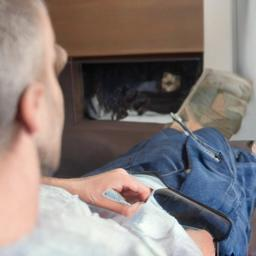
\includegraphics[width=0.24\linewidth]{figs/samples/cfg0.0_prompt_37_image_3.jpg}\,%
        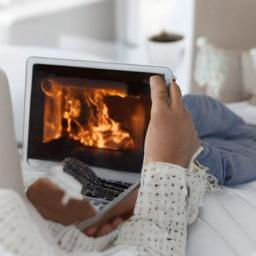
\includegraphics[width=0.24\linewidth]{figs/samples/cfg0.0_prompt_37_image_5.jpg}\,%
        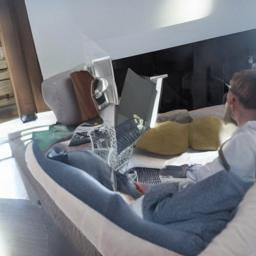
\includegraphics[width=0.24\linewidth]{figs/samples/cfg0.0_prompt_37_image_6.jpg}\,%
        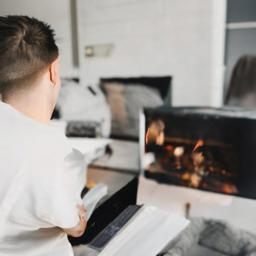
\includegraphics[width=0.24\linewidth]{figs/samples/cfg0.0_prompt_37_image_7.jpg}\\
        \rotatebox{90}{\;\;\; $w=1.0$}\,%
        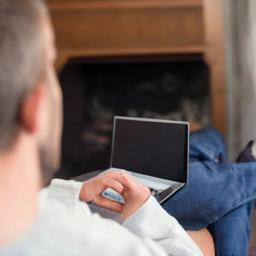
\includegraphics[width=0.24\linewidth]{figs/samples/cfg1.0_prompt_37_image_3.jpg}\,%
        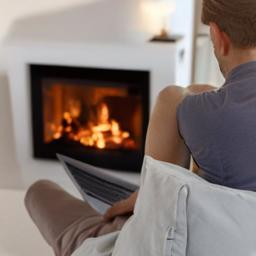
\includegraphics[width=0.24\linewidth]{figs/samples/cfg1.0_prompt_37_image_5.jpg}\,%
        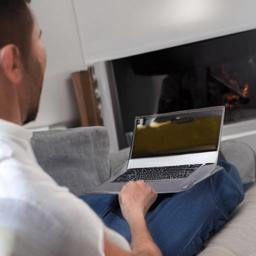
\includegraphics[width=0.24\linewidth]{figs/samples/cfg1.0_prompt_37_image_6.jpg}\,%
        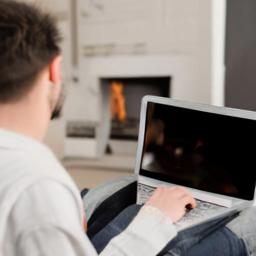
\includegraphics[width=0.24\linewidth]{figs/samples/cfg1.0_prompt_37_image_7.jpg}\\
        \rotatebox{90}{\;\;\; $w=4.0$}\,%
        
\includegraphics[width=0.24\linewidth]{figs/samples/cfg4.0_prompt_37_image_3.jpg}\,%
        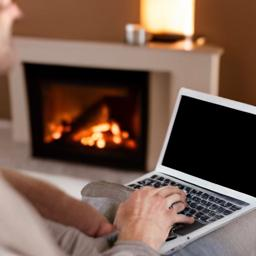
\includegraphics[width=0.24\linewidth]{figs/samples/cfg4.0_prompt_37_image_5.jpg}\,%
        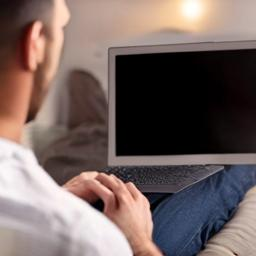
\includegraphics[width=0.24\linewidth]{figs/samples/cfg4.0_prompt_37_image_6.jpg}\,%
        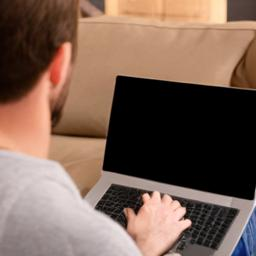
\includegraphics[width=0.24\linewidth]{figs/samples/cfg4.0_prompt_37_image_7.jpg}
        \caption*{Text prompt: ``\textit{Man sitting on sofa at home in front of fireplace and using laptop computer, rear view}''}
    \end{subfigure}\hfill
    \begin{subfigure}[t]{0.49\linewidth}
        \centering
        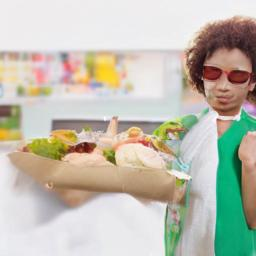
\includegraphics[width=0.24\linewidth]{figs/samples/cfg0.0_prompt_74_image_6.jpg}\,%
        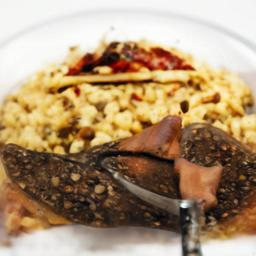
\includegraphics[width=0.24\linewidth]{figs/samples/cfg0.0_prompt_74_image_7.jpg}\,%
        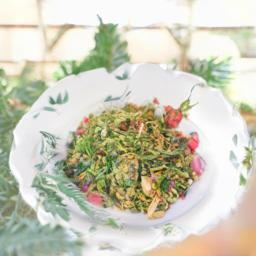
\includegraphics[width=0.24\linewidth]{figs/samples/cfg0.0_prompt_74_image_8.jpg}\,%
        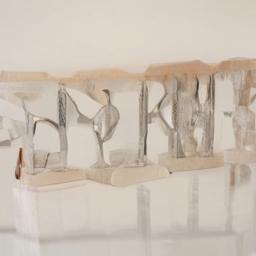
\includegraphics[width=0.24\linewidth]{figs/samples/cfg0.0_prompt_74_image_9.jpg}\\
        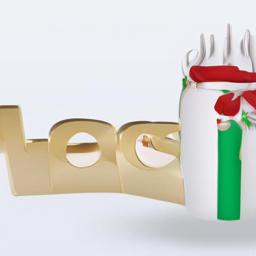
\includegraphics[width=0.24\linewidth]{figs/samples/cfg1.0_prompt_74_image_6.jpg}\,%
        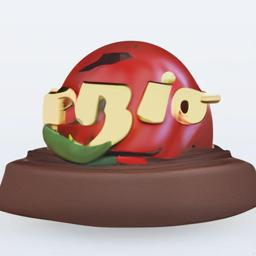
\includegraphics[width=0.24\linewidth]{figs/samples/cfg1.0_prompt_74_image_7.jpg}\,%
        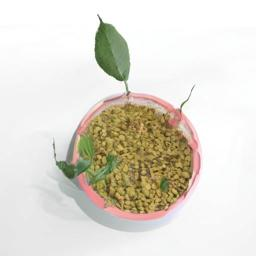
\includegraphics[width=0.24\linewidth]{figs/samples/cfg1.0_prompt_74_image_8.jpg}\,%
        
\includegraphics[width=0.24\linewidth]{figs/samples/cfg1.0_prompt_74_image_9.jpg}\\
        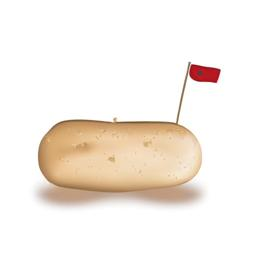
\includegraphics[width=0.24\linewidth]{figs/samples/cfg4.0_prompt_74_image_6.jpg}\,%
        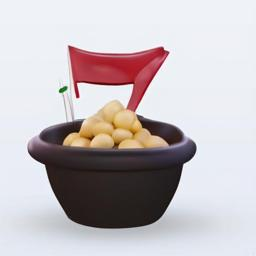
\includegraphics[width=0.24\linewidth]{figs/samples/cfg4.0_prompt_74_image_7.jpg}\,%
        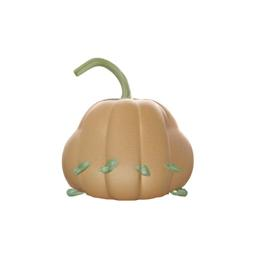
\includegraphics[width=0.24\linewidth]{figs/samples/cfg4.0_prompt_74_image_8.jpg}\,%
        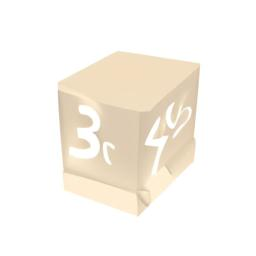
\includegraphics[width=0.24\linewidth]{figs/samples/cfg4.0_prompt_74_image_9.jpg}
        \caption*{Text prompt: ``\textit{3D World Food Day Morocco}''}
    \end{subfigure}
    \caption{
    Generated samples from varying classifier-free guidance weights, from the pre-trained Flow Matching model. 
    Corresponding samples from the fine-tuned model can be found in \Cref{fig:ablation_tradeoff_cfg}. 
    }
    \label{fig:ablation_tradeoff_cfg_base}
\end{figure}


\begin{figure}[h!]
    \centering
    \begin{subfigure}[t]{0.32\linewidth}
    \centering
    \caption*{Base Flow Matching model}
	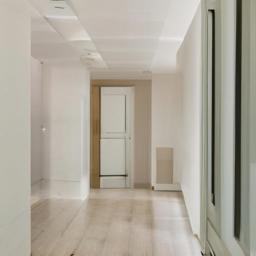
\includegraphics[width=0.320\linewidth]{figs/samples_appendix_3/base_cfg_2_ode_prompt_6_image_1.jpg}\;%
	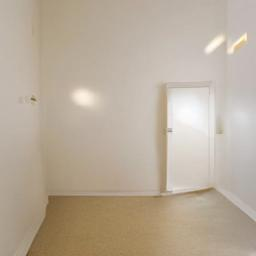
\includegraphics[width=0.320\linewidth]{figs/samples_appendix_3/base_cfg_2_ode_prompt_6_image_2.jpg}\;%
	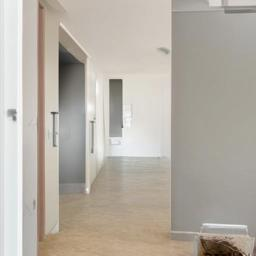
\includegraphics[width=0.320\linewidth]{figs/samples_appendix_3/base_cfg_2_ode_prompt_6_image_3.jpg}\\ 
	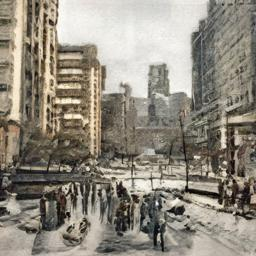
\includegraphics[width=0.320\linewidth]{figs/samples_appendix_3/base_cfg_2_ode_prompt_14_image_1.jpg}\;%
	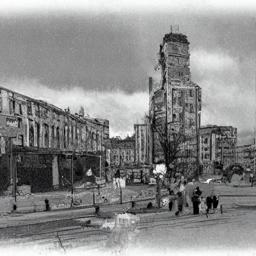
\includegraphics[width=0.320\linewidth]{figs/samples_appendix_3/base_cfg_2_ode_prompt_14_image_2.jpg}\;%
	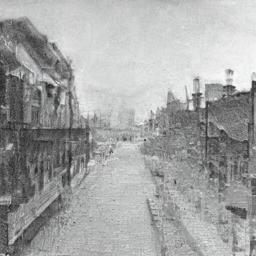
\includegraphics[width=0.320\linewidth]{figs/samples_appendix_3/base_cfg_2_ode_prompt_14_image_3.jpg}\\ 
	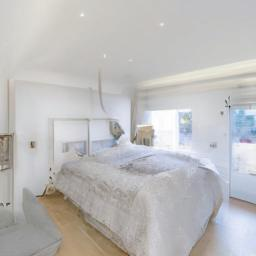
\includegraphics[width=0.320\linewidth]{figs/samples_appendix_3/base_cfg_2_ode_prompt_19_image_1.jpg}\;%
	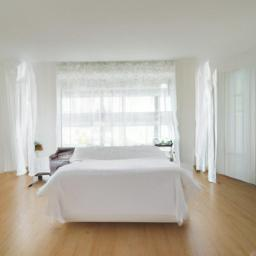
\includegraphics[width=0.320\linewidth]{figs/samples_appendix_3/base_cfg_2_ode_prompt_19_image_2.jpg}\;%
	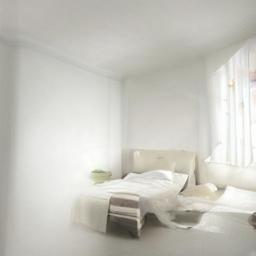
\includegraphics[width=0.320\linewidth]{figs/samples_appendix_3/base_cfg_2_ode_prompt_19_image_3.jpg}\\ 
	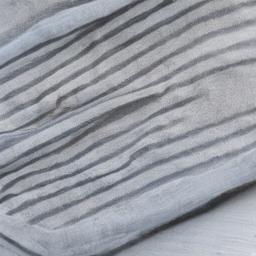
\includegraphics[width=0.320\linewidth]{figs/samples_appendix_3/base_cfg_2_ode_prompt_28_image_1.jpg}\;%
	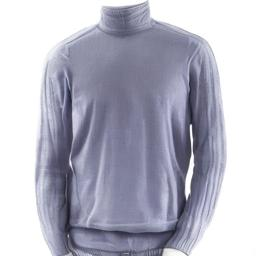
\includegraphics[width=0.320\linewidth]{figs/samples_appendix_3/base_cfg_2_ode_prompt_28_image_2.jpg}\;%
	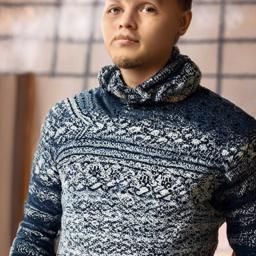
\includegraphics[width=0.320\linewidth]{figs/samples_appendix_3/base_cfg_2_ode_prompt_28_image_3.jpg}\\ 
	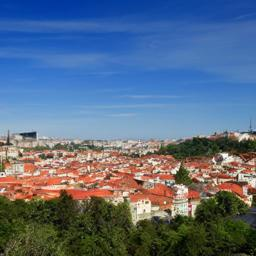
\includegraphics[width=0.320\linewidth]{figs/samples_appendix_3/base_cfg_2_ode_prompt_34_image_1.jpg}\;%
	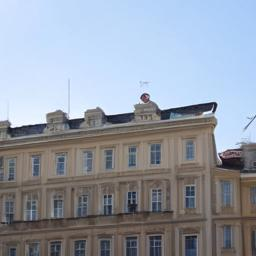
\includegraphics[width=0.320\linewidth]{figs/samples_appendix_3/base_cfg_2_ode_prompt_34_image_2.jpg}\;%
	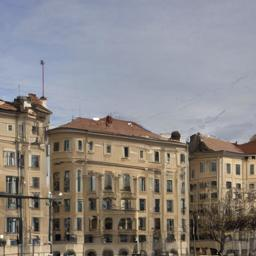
\includegraphics[width=0.320\linewidth]{figs/samples_appendix_3/base_cfg_2_ode_prompt_34_image_3.jpg}\\ 
	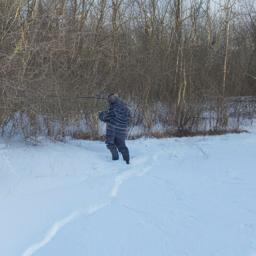
\includegraphics[width=0.320\linewidth]{figs/samples_appendix_3/base_cfg_2_ode_prompt_65_image_1.jpg}\;%
	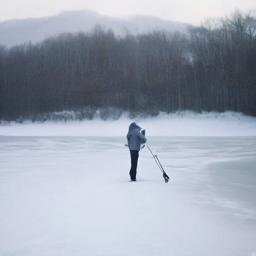
\includegraphics[width=0.320\linewidth]{figs/samples_appendix_3/base_cfg_2_ode_prompt_65_image_2.jpg}\;%
	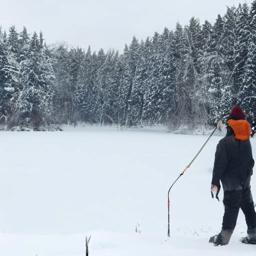
\includegraphics[width=0.320\linewidth]{figs/samples_appendix_3/base_cfg_2_ode_prompt_65_image_3.jpg}\\ 
	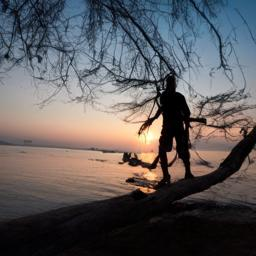
\includegraphics[width=0.320\linewidth]{figs/samples_appendix_3/base_cfg_2_ode_prompt_69_image_1.jpg}\;%
	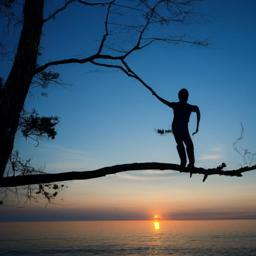
\includegraphics[width=0.320\linewidth]{figs/samples_appendix_3/base_cfg_2_ode_prompt_69_image_2.jpg}\;%
	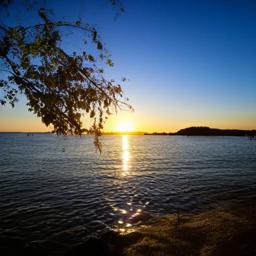
\includegraphics[width=0.320\linewidth]{figs/samples_appendix_3/base_cfg_2_ode_prompt_69_image_3.jpg}\\ 
	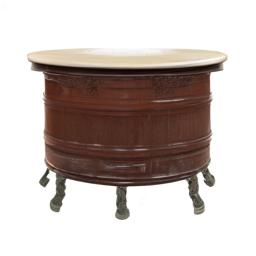
\includegraphics[width=0.320\linewidth]{figs/samples_appendix_3/base_cfg_2_ode_prompt_73_image_1.jpg}\;%
	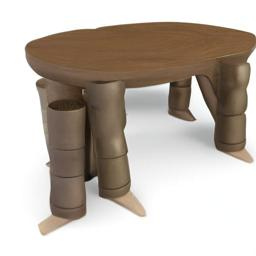
\includegraphics[width=0.320\linewidth]{figs/samples_appendix_3/base_cfg_2_ode_prompt_73_image_2.jpg}\;%
	\includegraphics[width=0.320\linewidth]{figs/samples_appendix_3/base_cfg_2_ode_prompt_73_image_3.jpg}\\ 
	\includegraphics[width=0.320\linewidth]{figs/samples_appendix_3/base_cfg_2_ode_prompt_75_image_1.jpg}\;%
	\includegraphics[width=0.320\linewidth]{figs/samples_appendix_3/base_cfg_2_ode_prompt_75_image_2.jpg}\;%
	\includegraphics[width=0.320\linewidth]{figs/samples_appendix_3/base_cfg_2_ode_prompt_75_image_3.jpg}\\ 
	\includegraphics[width=0.320\linewidth]{figs/samples_appendix_3/base_cfg_2_ode_prompt_90_image_1.jpg}\;%
	\includegraphics[width=0.320\linewidth]{figs/samples_appendix_3/base_cfg_2_ode_prompt_90_image_2.jpg}\;%
	\includegraphics[width=0.320\linewidth]{figs/samples_appendix_3/base_cfg_2_ode_prompt_90_image_3.jpg}
    \end{subfigure}\hfill
    \begin{subfigure}[t]{0.32\linewidth}
    \centering
    \caption*{Adjoint Matching (Ours)}
	\includegraphics[width=0.320\linewidth]{figs/samples_appendix_3/adjmat_cfg_2_ode_prompt_6_image_1.jpg}\;%
	\includegraphics[width=0.320\linewidth]{figs/samples_appendix_3/adjmat_cfg_2_ode_prompt_6_image_2.jpg}\;%
	\includegraphics[width=0.320\linewidth]{figs/samples_appendix_3/adjmat_cfg_2_ode_prompt_6_image_3.jpg}\\ 
	\includegraphics[width=0.320\linewidth]{figs/samples_appendix_3/adjmat_cfg_2_ode_prompt_14_image_1.jpg}\;%
	\includegraphics[width=0.320\linewidth]{figs/samples_appendix_3/adjmat_cfg_2_ode_prompt_14_image_2.jpg}\;%
	\includegraphics[width=0.320\linewidth]{figs/samples_appendix_3/adjmat_cfg_2_ode_prompt_14_image_3.jpg}\\ 
	\includegraphics[width=0.320\linewidth]{figs/samples_appendix_3/adjmat_cfg_2_ode_prompt_19_image_1.jpg}\;%
	\includegraphics[width=0.320\linewidth]{figs/samples_appendix_3/adjmat_cfg_2_ode_prompt_19_image_2.jpg}\;%
	\includegraphics[width=0.320\linewidth]{figs/samples_appendix_3/adjmat_cfg_2_ode_prompt_19_image_3.jpg}\\ 
	\includegraphics[width=0.320\linewidth]{figs/samples_appendix_3/adjmat_cfg_2_ode_prompt_28_image_1.jpg}\;%
	\includegraphics[width=0.320\linewidth]{figs/samples_appendix_3/adjmat_cfg_2_ode_prompt_28_image_2.jpg}\;%
	\includegraphics[width=0.320\linewidth]{figs/samples_appendix_3/adjmat_cfg_2_ode_prompt_28_image_3.jpg}\\ 
	\includegraphics[width=0.320\linewidth]{figs/samples_appendix_3/adjmat_cfg_2_ode_prompt_34_image_1.jpg}\;%
	\includegraphics[width=0.320\linewidth]{figs/samples_appendix_3/adjmat_cfg_2_ode_prompt_34_image_2.jpg}\;%
	\includegraphics[width=0.320\linewidth]{figs/samples_appendix_3/adjmat_cfg_2_ode_prompt_34_image_3.jpg}\\ 
	\includegraphics[width=0.320\linewidth]{figs/samples_appendix_3/adjmat_cfg_2_ode_prompt_65_image_1.jpg}\;%
	\includegraphics[width=0.320\linewidth]{figs/samples_appendix_3/adjmat_cfg_2_ode_prompt_65_image_2.jpg}\;%
	\includegraphics[width=0.320\linewidth]{figs/samples_appendix_3/adjmat_cfg_2_ode_prompt_65_image_3.jpg}\\ 
	\includegraphics[width=0.320\linewidth]{figs/samples_appendix_3/adjmat_cfg_2_ode_prompt_69_image_1.jpg}\;%
	\includegraphics[width=0.320\linewidth]{figs/samples_appendix_3/adjmat_cfg_2_ode_prompt_69_image_2.jpg}\;%
	\includegraphics[width=0.320\linewidth]{figs/samples_appendix_3/adjmat_cfg_2_ode_prompt_69_image_3.jpg}\\ 
	\includegraphics[width=0.320\linewidth]{figs/samples_appendix_3/adjmat_cfg_2_ode_prompt_73_image_1.jpg}\;%
	\includegraphics[width=0.320\linewidth]{figs/samples_appendix_3/adjmat_cfg_2_ode_prompt_73_image_2.jpg}\;%
	\includegraphics[width=0.320\linewidth]{figs/samples_appendix_3/adjmat_cfg_2_ode_prompt_73_image_3.jpg}\\ 
	\includegraphics[width=0.320\linewidth]{figs/samples_appendix_3/adjmat_cfg_2_ode_prompt_75_image_1.jpg}\;%
	\includegraphics[width=0.320\linewidth]{figs/samples_appendix_3/adjmat_cfg_2_ode_prompt_75_image_2.jpg}\;%
	\includegraphics[width=0.320\linewidth]{figs/samples_appendix_3/adjmat_cfg_2_ode_prompt_75_image_3.jpg}\\ 
	\includegraphics[width=0.320\linewidth]{figs/samples_appendix_3/adjmat_cfg_2_ode_prompt_90_image_1.jpg}\;%
	\includegraphics[width=0.320\linewidth]{figs/samples_appendix_3/adjmat_cfg_2_ode_prompt_90_image_2.jpg}\;%
	\includegraphics[width=0.320\linewidth]{figs/samples_appendix_3/adjmat_cfg_2_ode_prompt_90_image_3.jpg}
    \end{subfigure}\hfill
    \begin{subfigure}[t]{0.32\linewidth}
    \centering
    \caption*{DRaFT-1}
	\includegraphics[width=0.320\linewidth]{figs/samples_appendix_3/draft1k_cfg_2_ode_prompt_6_image_1.jpg}\;%
	\includegraphics[width=0.320\linewidth]{figs/samples_appendix_3/draft1k_cfg_2_ode_prompt_6_image_2.jpg}\;%
	\includegraphics[width=0.320\linewidth]{figs/samples_appendix_3/draft1k_cfg_2_ode_prompt_6_image_3.jpg}\\ 
	\includegraphics[width=0.320\linewidth]{figs/samples_appendix_3/draft1k_cfg_2_ode_prompt_14_image_1.jpg}\;%
	\includegraphics[width=0.320\linewidth]{figs/samples_appendix_3/draft1k_cfg_2_ode_prompt_14_image_2.jpg}\;%
	\includegraphics[width=0.320\linewidth]{figs/samples_appendix_3/draft1k_cfg_2_ode_prompt_14_image_3.jpg}\\ 
	\includegraphics[width=0.320\linewidth]{figs/samples_appendix_3/draft1k_cfg_2_ode_prompt_19_image_1.jpg}\;%
	\includegraphics[width=0.320\linewidth]{figs/samples_appendix_3/draft1k_cfg_2_ode_prompt_19_image_2.jpg}\;%
	\includegraphics[width=0.320\linewidth]{figs/samples_appendix_3/draft1k_cfg_2_ode_prompt_19_image_3.jpg}\\ 
	\includegraphics[width=0.320\linewidth]{figs/samples_appendix_3/draft1k_cfg_2_ode_prompt_28_image_1.jpg}\;%
	\includegraphics[width=0.320\linewidth]{figs/samples_appendix_3/draft1k_cfg_2_ode_prompt_28_image_2.jpg}\;%
	\includegraphics[width=0.320\linewidth]{figs/samples_appendix_3/draft1k_cfg_2_ode_prompt_28_image_3.jpg}\\ 
	\includegraphics[width=0.320\linewidth]{figs/samples_appendix_3/draft1k_cfg_2_ode_prompt_34_image_1.jpg}\;%
	\includegraphics[width=0.320\linewidth]{figs/samples_appendix_3/draft1k_cfg_2_ode_prompt_34_image_2.jpg}\;%
	\includegraphics[width=0.320\linewidth]{figs/samples_appendix_3/draft1k_cfg_2_ode_prompt_34_image_3.jpg}\\ 
	\includegraphics[width=0.320\linewidth]{figs/samples_appendix_3/draft1k_cfg_2_ode_prompt_65_image_1.jpg}\;%
	\includegraphics[width=0.320\linewidth]{figs/samples_appendix_3/draft1k_cfg_2_ode_prompt_65_image_2.jpg}\;%
	\includegraphics[width=0.320\linewidth]{figs/samples_appendix_3/draft1k_cfg_2_ode_prompt_65_image_3.jpg}\\ 
	\includegraphics[width=0.320\linewidth]{figs/samples_appendix_3/draft1k_cfg_2_ode_prompt_69_image_1.jpg}\;%
	\includegraphics[width=0.320\linewidth]{figs/samples_appendix_3/draft1k_cfg_2_ode_prompt_69_image_2.jpg}\;%
	\includegraphics[width=0.320\linewidth]{figs/samples_appendix_3/draft1k_cfg_2_ode_prompt_69_image_3.jpg}\\ 
	\includegraphics[width=0.320\linewidth]{figs/samples_appendix_3/draft1k_cfg_2_ode_prompt_73_image_1.jpg}\;%
	\includegraphics[width=0.320\linewidth]{figs/samples_appendix_3/draft1k_cfg_2_ode_prompt_73_image_2.jpg}\;%
	\includegraphics[width=0.320\linewidth]{figs/samples_appendix_3/draft1k_cfg_2_ode_prompt_73_image_3.jpg}\\ 
	\includegraphics[width=0.320\linewidth]{figs/samples_appendix_3/draft1k_cfg_2_ode_prompt_75_image_1.jpg}\;%
	\includegraphics[width=0.320\linewidth]{figs/samples_appendix_3/draft1k_cfg_2_ode_prompt_75_image_2.jpg}\;%
	\includegraphics[width=0.320\linewidth]{figs/samples_appendix_3/draft1k_cfg_2_ode_prompt_75_image_3.jpg}\\ 
	\includegraphics[width=0.320\linewidth]{figs/samples_appendix_3/draft1k_cfg_2_ode_prompt_90_image_1.jpg}\;%
	\includegraphics[width=0.320\linewidth]{figs/samples_appendix_3/draft1k_cfg_2_ode_prompt_90_image_2.jpg}\;%
	\includegraphics[width=0.320\linewidth]{figs/samples_appendix_3/draft1k_cfg_2_ode_prompt_90_image_3.jpg}
    \end{subfigure}
    \caption{
    Generated samples with classifier-free guidance ($w=1$) and $\sigma(t)=0$ across ten selected prompts.  Each row corresponds to a different prompt and each image corresponds to a different random seed consistent across models.
    }
    \label{fig:image_comparison_v2}
\end{figure}

\begin{figure}[h!]
\centering
    \begin{subfigure}[t]{0.32\linewidth}
    \centering
    \caption*{Base Flow Matching model}
    	\includegraphics[width=0.32\linewidth]{figs/samples_appendix_4/base_cfg_2_ode_prompt_12_image_0.jpg}\;%
    	\includegraphics[width=0.32\linewidth]{figs/samples_appendix_4/base_cfg_2_ode_prompt_12_image_1.jpg}\;%
    	\includegraphics[width=0.32\linewidth]{figs/samples_appendix_4/base_cfg_2_ode_prompt_12_image_2.jpg}\\ 
    	\includegraphics[width=0.32\linewidth]{figs/samples_appendix_4/base_cfg_2_ode_prompt_16_image_0.jpg}\;%
    	\includegraphics[width=0.32\linewidth]{figs/samples_appendix_4/base_cfg_2_ode_prompt_16_image_1.jpg}\;%
    	\includegraphics[width=0.32\linewidth]{figs/samples_appendix_4/base_cfg_2_ode_prompt_16_image_2.jpg}\\ 
    	\includegraphics[width=0.32\linewidth]{figs/samples_appendix_4/base_cfg_2_ode_prompt_17_image_0.jpg}\;%
    	\includegraphics[width=0.32\linewidth]{figs/samples_appendix_4/base_cfg_2_ode_prompt_17_image_1.jpg}\;%
    	\includegraphics[width=0.32\linewidth]{figs/samples_appendix_4/base_cfg_2_ode_prompt_17_image_2.jpg}\\ 
    	\includegraphics[width=0.32\linewidth]{figs/samples_appendix_4/base_cfg_2_ode_prompt_21_image_0.jpg}\;%
    	\includegraphics[width=0.32\linewidth]{figs/samples_appendix_4/base_cfg_2_ode_prompt_21_image_1.jpg}\;%
    	\includegraphics[width=0.32\linewidth]{figs/samples_appendix_4/base_cfg_2_ode_prompt_21_image_2.jpg}\\ 
    	\includegraphics[width=0.32\linewidth]{figs/samples_appendix_4/base_cfg_2_ode_prompt_33_image_0.jpg}\;%
    	\includegraphics[width=0.32\linewidth]{figs/samples_appendix_4/base_cfg_2_ode_prompt_33_image_1.jpg}\;%
    	\includegraphics[width=0.32\linewidth]{figs/samples_appendix_4/base_cfg_2_ode_prompt_33_image_2.jpg}\\ 
    	\includegraphics[width=0.32\linewidth]{figs/samples_appendix_4/base_cfg_2_ode_prompt_35_image_0.jpg}\;%
    	\includegraphics[width=0.32\linewidth]{figs/samples_appendix_4/base_cfg_2_ode_prompt_35_image_1.jpg}\;%
    	\includegraphics[width=0.32\linewidth]{figs/samples_appendix_4/base_cfg_2_ode_prompt_35_image_2.jpg}\\ 
    	\includegraphics[width=0.32\linewidth]{figs/samples_appendix_4/base_cfg_2_ode_prompt_51_image_0.jpg}\;%
    	\includegraphics[width=0.32\linewidth]{figs/samples_appendix_4/base_cfg_2_ode_prompt_51_image_1.jpg}\;%
    	\includegraphics[width=0.32\linewidth]{figs/samples_appendix_4/base_cfg_2_ode_prompt_51_image_2.jpg}\\ 
    	\includegraphics[width=0.32\linewidth]{figs/samples_appendix_4/base_cfg_2_ode_prompt_58_image_0.jpg}\;%
    	\includegraphics[width=0.32\linewidth]{figs/samples_appendix_4/base_cfg_2_ode_prompt_58_image_1.jpg}\;%
    	\includegraphics[width=0.32\linewidth]{figs/samples_appendix_4/base_cfg_2_ode_prompt_58_image_2.jpg}\\ 
    	\includegraphics[width=0.32\linewidth]{figs/samples_appendix_4/base_cfg_2_ode_prompt_61_image_0.jpg}\;%
    	\includegraphics[width=0.32\linewidth]{figs/samples_appendix_4/base_cfg_2_ode_prompt_61_image_1.jpg}\;%
    	\includegraphics[width=0.32\linewidth]{figs/samples_appendix_4/base_cfg_2_ode_prompt_61_image_2.jpg}\\ 
    	\includegraphics[width=0.32\linewidth]{figs/samples_appendix_4/base_cfg_2_ode_prompt_63_image_0.jpg}\;%
    	\includegraphics[width=0.32\linewidth]{figs/samples_appendix_4/base_cfg_2_ode_prompt_63_image_1.jpg}\;%
    	\includegraphics[width=0.32\linewidth]{figs/samples_appendix_4/base_cfg_2_ode_prompt_63_image_2.jpg}
    \end{subfigure}\hfill
    \begin{subfigure}[t]{0.32\linewidth}
    \centering
    \caption*{Adjoint Matching (Ours)}
    	\includegraphics[width=0.32\linewidth]{figs/samples_appendix_4/adjmat_cfg_2_ode_prompt_12_image_0.jpg}\;%
    	\includegraphics[width=0.32\linewidth]{figs/samples_appendix_4/adjmat_cfg_2_ode_prompt_12_image_1.jpg}\;%
    	\includegraphics[width=0.32\linewidth]{figs/samples_appendix_4/adjmat_cfg_2_ode_prompt_12_image_2.jpg}\\ 
    	\includegraphics[width=0.32\linewidth]{figs/samples_appendix_4/adjmat_cfg_2_ode_prompt_16_image_0.jpg}\;%
    	\includegraphics[width=0.32\linewidth]{figs/samples_appendix_4/adjmat_cfg_2_ode_prompt_16_image_1.jpg}\;%
    	\includegraphics[width=0.32\linewidth]{figs/samples_appendix_4/adjmat_cfg_2_ode_prompt_16_image_2.jpg}\\ 
    	\includegraphics[width=0.32\linewidth]{figs/samples_appendix_4/adjmat_cfg_2_ode_prompt_17_image_0.jpg}\;%
    	\includegraphics[width=0.32\linewidth]{figs/samples_appendix_4/adjmat_cfg_2_ode_prompt_17_image_1.jpg}\;%
    	\includegraphics[width=0.32\linewidth]{figs/samples_appendix_4/adjmat_cfg_2_ode_prompt_17_image_2.jpg}\\ 
    	\includegraphics[width=0.32\linewidth]{figs/samples_appendix_4/adjmat_cfg_2_ode_prompt_21_image_0.jpg}\;%
    	\includegraphics[width=0.32\linewidth]{figs/samples_appendix_4/adjmat_cfg_2_ode_prompt_21_image_1.jpg}\;%
    	\includegraphics[width=0.32\linewidth]{figs/samples_appendix_4/adjmat_cfg_2_ode_prompt_21_image_2.jpg}\\ 
    	\includegraphics[width=0.32\linewidth]{figs/samples_appendix_4/adjmat_cfg_2_ode_prompt_33_image_0.jpg}\;%
    	\includegraphics[width=0.32\linewidth]{figs/samples_appendix_4/adjmat_cfg_2_ode_prompt_33_image_1.jpg}\;%
    	\includegraphics[width=0.32\linewidth]{figs/samples_appendix_4/adjmat_cfg_2_ode_prompt_33_image_2.jpg}\\ 
    	\includegraphics[width=0.32\linewidth]{figs/samples_appendix_4/adjmat_cfg_2_ode_prompt_35_image_0.jpg}\;%
    	\includegraphics[width=0.32\linewidth]{figs/samples_appendix_4/adjmat_cfg_2_ode_prompt_35_image_1.jpg}\;%
    	\includegraphics[width=0.32\linewidth]{figs/samples_appendix_4/adjmat_cfg_2_ode_prompt_35_image_2.jpg}\\ 
    	\includegraphics[width=0.32\linewidth]{figs/samples_appendix_4/adjmat_cfg_2_ode_prompt_51_image_0.jpg}\;%
    	\includegraphics[width=0.32\linewidth]{figs/samples_appendix_4/adjmat_cfg_2_ode_prompt_51_image_1.jpg}\;%
    	\includegraphics[width=0.32\linewidth]{figs/samples_appendix_4/adjmat_cfg_2_ode_prompt_51_image_2.jpg}\\ 
    	\includegraphics[width=0.32\linewidth]{figs/samples_appendix_4/adjmat_cfg_2_ode_prompt_58_image_0.jpg}\;%
    	\includegraphics[width=0.32\linewidth]{figs/samples_appendix_4/adjmat_cfg_2_ode_prompt_58_image_1.jpg}\;%
    	\includegraphics[width=0.32\linewidth]{figs/samples_appendix_4/adjmat_cfg_2_ode_prompt_58_image_2.jpg}\\ 
    	\includegraphics[width=0.32\linewidth]{figs/samples_appendix_4/adjmat_cfg_2_ode_prompt_61_image_0.jpg}\;%
    	\includegraphics[width=0.32\linewidth]{figs/samples_appendix_4/adjmat_cfg_2_ode_prompt_61_image_1.jpg}\;%
    	\includegraphics[width=0.32\linewidth]{figs/samples_appendix_4/adjmat_cfg_2_ode_prompt_61_image_2.jpg}\\ 
    	\includegraphics[width=0.32\linewidth]{figs/samples_appendix_4/adjmat_cfg_2_ode_prompt_63_image_0.jpg}\;%
    	\includegraphics[width=0.32\linewidth]{figs/samples_appendix_4/adjmat_cfg_2_ode_prompt_63_image_1.jpg}\;%
    	\includegraphics[width=0.32\linewidth]{figs/samples_appendix_4/adjmat_cfg_2_ode_prompt_63_image_2.jpg}
    \end{subfigure}\hfill
    \begin{subfigure}[t]{0.32\linewidth}
    \centering
    \caption*{DRaFT-1}
    	\includegraphics[width=0.32\linewidth]{figs/samples_appendix_4/draft1k_cfg_2_ode_prompt_12_image_0.jpg}\;%
    	\includegraphics[width=0.32\linewidth]{figs/samples_appendix_4/draft1k_cfg_2_ode_prompt_12_image_1.jpg}\;%
    	\includegraphics[width=0.32\linewidth]{figs/samples_appendix_4/draft1k_cfg_2_ode_prompt_12_image_2.jpg}\\ 
    	\includegraphics[width=0.32\linewidth]{figs/samples_appendix_4/draft1k_cfg_2_ode_prompt_16_image_0.jpg}\;%
    	\includegraphics[width=0.32\linewidth]{figs/samples_appendix_4/draft1k_cfg_2_ode_prompt_16_image_1.jpg}\;%
    	\includegraphics[width=0.32\linewidth]{figs/samples_appendix_4/draft1k_cfg_2_ode_prompt_16_image_2.jpg}\\ 
    	\includegraphics[width=0.32\linewidth]{figs/samples_appendix_4/draft1k_cfg_2_ode_prompt_17_image_0.jpg}\;%
    	\includegraphics[width=0.32\linewidth]{figs/samples_appendix_4/draft1k_cfg_2_ode_prompt_17_image_1.jpg}\;%
    	\includegraphics[width=0.32\linewidth]{figs/samples_appendix_4/draft1k_cfg_2_ode_prompt_17_image_2.jpg}\\ 
    	\includegraphics[width=0.32\linewidth]{figs/samples_appendix_4/draft1k_cfg_2_ode_prompt_21_image_0.jpg}\;%
    	\includegraphics[width=0.32\linewidth]{figs/samples_appendix_4/draft1k_cfg_2_ode_prompt_21_image_1.jpg}\;%
    	\includegraphics[width=0.32\linewidth]{figs/samples_appendix_4/draft1k_cfg_2_ode_prompt_21_image_2.jpg}\\ 
    	\includegraphics[width=0.32\linewidth]{figs/samples_appendix_4/draft1k_cfg_2_ode_prompt_33_image_0.jpg}\;%
    	\includegraphics[width=0.32\linewidth]{figs/samples_appendix_4/draft1k_cfg_2_ode_prompt_33_image_1.jpg}\;%
    	\includegraphics[width=0.32\linewidth]{figs/samples_appendix_4/draft1k_cfg_2_ode_prompt_33_image_2.jpg}\\ 
    	\includegraphics[width=0.32\linewidth]{figs/samples_appendix_4/draft1k_cfg_2_ode_prompt_35_image_0.jpg}\;%
    	\includegraphics[width=0.32\linewidth]{figs/samples_appendix_4/draft1k_cfg_2_ode_prompt_35_image_1.jpg}\;%
    	\includegraphics[width=0.32\linewidth]{figs/samples_appendix_4/draft1k_cfg_2_ode_prompt_35_image_2.jpg}\\ 
    	\includegraphics[width=0.32\linewidth]{figs/samples_appendix_4/draft1k_cfg_2_ode_prompt_51_image_0.jpg}\;%
    	\includegraphics[width=0.32\linewidth]{figs/samples_appendix_4/draft1k_cfg_2_ode_prompt_51_image_1.jpg}\;%
    	\includegraphics[width=0.32\linewidth]{figs/samples_appendix_4/draft1k_cfg_2_ode_prompt_51_image_2.jpg}\\ 
    	\includegraphics[width=0.32\linewidth]{figs/samples_appendix_4/draft1k_cfg_2_ode_prompt_58_image_0.jpg}\;%
    	\includegraphics[width=0.32\linewidth]{figs/samples_appendix_4/draft1k_cfg_2_ode_prompt_58_image_1.jpg}\;%
    	\includegraphics[width=0.32\linewidth]{figs/samples_appendix_4/draft1k_cfg_2_ode_prompt_58_image_2.jpg}\\ 
    	\includegraphics[width=0.32\linewidth]{figs/samples_appendix_4/draft1k_cfg_2_ode_prompt_61_image_0.jpg}\;%
    	\includegraphics[width=0.32\linewidth]{figs/samples_appendix_4/draft1k_cfg_2_ode_prompt_61_image_1.jpg}\;%
    	\includegraphics[width=0.32\linewidth]{figs/samples_appendix_4/draft1k_cfg_2_ode_prompt_61_image_2.jpg}\\ 
    	\includegraphics[width=0.32\linewidth]{figs/samples_appendix_4/draft1k_cfg_2_ode_prompt_63_image_0.jpg}\;%
    	\includegraphics[width=0.32\linewidth]{figs/samples_appendix_4/draft1k_cfg_2_ode_prompt_63_image_1.jpg}\;%
    	\includegraphics[width=0.32\linewidth]{figs/samples_appendix_4/draft1k_cfg_2_ode_prompt_63_image_2.jpg}
    \end{subfigure}
    \caption{
    Generated samples with classifier-free guidance ($w=1$) and $\sigma(t) = 0$ across ten selected prompts with people.  Each row corresponds to a different prompt and each image corresponds to a different random seed consistent across models.
    }
    \label{fig:image_comparison_people}
\end{figure}

\begin{figure}[!htb]
    \centering
    \begin{tabular}{>{\centering\arraybackslash}m{0.3cm} m{0.96\linewidth}}
        \rotatebox{90}{\parbox{2cm}{\centering\footnotesize None (Base)}} &
        \includegraphics[width=0.135\linewidth]{figs/samples_appendix_5/none_ode/prompt_606.jpg}
    	\includegraphics[width=0.135\linewidth]{figs/samples_appendix_5/none_ode/prompt_576.jpg}
    	\includegraphics[width=0.135\linewidth]{figs/samples_appendix_5/none_ode/prompt_554.jpg}
    	\includegraphics[width=0.135\linewidth]{figs/samples_appendix_5/none_ode/prompt_345.jpg}
    	\includegraphics[width=0.135\linewidth]{figs/samples_appendix_5/none_ode/prompt_162.jpg}
    	\includegraphics[width=0.135\linewidth]{figs/samples_appendix_5/none_ode/prompt_94.jpg}
    	\includegraphics[width=0.135\linewidth]{figs/samples_appendix_5/none_ode/prompt_143.jpg} \\

        \rotatebox{90}{\parbox{2cm}{\centering\footnotesize DRaFT-1}} &
        \includegraphics[width=0.135\linewidth]{figs/samples_appendix_5/draft1_ode/prompt_606.jpg}
    	\includegraphics[width=0.135\linewidth]{figs/samples_appendix_5/draft1_ode/prompt_576.jpg}
    	\includegraphics[width=0.135\linewidth]{figs/samples_appendix_5/draft1_ode/prompt_554.jpg}
    	\includegraphics[width=0.135\linewidth]{figs/samples_appendix_5/draft1_ode/prompt_345.jpg}
    	\includegraphics[width=0.135\linewidth]{figs/samples_appendix_5/draft1_ode/prompt_162.jpg}
    	\includegraphics[width=0.135\linewidth]{figs/samples_appendix_5/draft1_ode/prompt_94.jpg}
    	\includegraphics[width=0.135\linewidth]{figs/samples_appendix_5/draft1_ode/prompt_143.jpg} \\

        \rotatebox{90}{\parbox{2cm}{\centering\footnotesize DRaFT-40}} &
        \includegraphics[width=0.135\linewidth]{figs/samples_appendix_5/draft40_ode/prompt_606.jpg}
    	\includegraphics[width=0.135\linewidth]{figs/samples_appendix_5/draft40_ode/prompt_576.jpg}
    	\includegraphics[width=0.135\linewidth]{figs/samples_appendix_5/draft40_ode/prompt_554.jpg}
    	\includegraphics[width=0.135\linewidth]{figs/samples_appendix_5/draft40_ode/prompt_345.jpg}
    	\includegraphics[width=0.135\linewidth]{figs/samples_appendix_5/draft40_ode/prompt_162.jpg}
    	\includegraphics[width=0.135\linewidth]{figs/samples_appendix_5/draft40_ode/prompt_94.jpg}
    	\includegraphics[width=0.135\linewidth]{figs/samples_appendix_5/draft40_ode/prompt_143.jpg} \\

        \rotatebox{90}{\parbox{2cm}{\centering\footnotesize ReFL}} &
        \includegraphics[width=0.135\linewidth]{figs/samples_appendix_5/refl_ode/prompt_606.jpg}
    	\includegraphics[width=0.135\linewidth]{figs/samples_appendix_5/refl_ode/prompt_576.jpg}
    	\includegraphics[width=0.135\linewidth]{figs/samples_appendix_5/refl_ode/prompt_554.jpg}
    	\includegraphics[width=0.135\linewidth]{figs/samples_appendix_5/refl_ode/prompt_345.jpg}
    	\includegraphics[width=0.135\linewidth]{figs/samples_appendix_5/refl_ode/prompt_162.jpg}
    	\includegraphics[width=0.135\linewidth]{figs/samples_appendix_5/refl_ode/prompt_94.jpg}
    	\includegraphics[width=0.135\linewidth]{figs/samples_appendix_5/refl_ode/prompt_143.jpg} \\

        \rotatebox{90}{\parbox{2cm}{\centering\footnotesize Cont. Adj.\\$\lambda = 12500$}} &
        \includegraphics[width=0.135\linewidth]{figs/samples_appendix_5/contadj_ode/prompt_606.jpg}
    	\includegraphics[width=0.135\linewidth]{figs/samples_appendix_5/contadj_ode/prompt_576.jpg}
    	\includegraphics[width=0.135\linewidth]{figs/samples_appendix_5/contadj_ode/prompt_554.jpg}
    	\includegraphics[width=0.135\linewidth]{figs/samples_appendix_5/contadj_ode/prompt_345.jpg}
    	\includegraphics[width=0.135\linewidth]{figs/samples_appendix_5/contadj_ode/prompt_162.jpg}
    	\includegraphics[width=0.135\linewidth]{figs/samples_appendix_5/contadj_ode/prompt_94.jpg}
    	\includegraphics[width=0.135\linewidth]{figs/samples_appendix_5/contadj_ode/prompt_143.jpg} \\

        \rotatebox{90}{\parbox{2cm}{\centering\footnotesize Disc. Adj.\\$\lambda = 12500$}} &
        \includegraphics[width=0.135\linewidth]{figs/samples_appendix_5/discadj_ode/prompt_606.jpg}
    	\includegraphics[width=0.135\linewidth]{figs/samples_appendix_5/discadj_ode/prompt_576.jpg}
    	\includegraphics[width=0.135\linewidth]{figs/samples_appendix_5/discadj_ode/prompt_554.jpg}
    	\includegraphics[width=0.135\linewidth]{figs/samples_appendix_5/discadj_ode/prompt_345.jpg}
    	\includegraphics[width=0.135\linewidth]{figs/samples_appendix_5/discadj_ode/prompt_162.jpg}
    	\includegraphics[width=0.135\linewidth]{figs/samples_appendix_5/discadj_ode/prompt_94.jpg}
    	\includegraphics[width=0.135\linewidth]{figs/samples_appendix_5/discadj_ode/prompt_143.jpg} \\
     
        \rotatebox{90}{\parbox{2cm}{\centering\footnotesize Adj. match.\\$\lambda = 1000$}} &
        \includegraphics[width=0.135\linewidth]{figs/samples_appendix_5/adjmat_1000_ode/prompt_606.jpg}
        \includegraphics[width=0.135\linewidth]{figs/samples_appendix_5/adjmat_1000_ode/prompt_576.jpg}
        \includegraphics[width=0.135\linewidth]{figs/samples_appendix_5/adjmat_1000_ode/prompt_554.jpg}
        \includegraphics[width=0.135\linewidth]{figs/samples_appendix_5/adjmat_1000_ode/prompt_345.jpg}
        \includegraphics[width=0.135\linewidth]{figs/samples_appendix_5/adjmat_1000_ode/prompt_162.jpg}
        \includegraphics[width=0.135\linewidth]{figs/samples_appendix_5/adjmat_1000_ode/prompt_94.jpg}
        \includegraphics[width=0.135\linewidth]{figs/samples_appendix_5/adjmat_1000_ode/prompt_143.jpg} \\

        \rotatebox{90}{\parbox{2cm}{\centering\footnotesize Adj. match.\\$\lambda = 2500$}} &
        \includegraphics[width=0.135\linewidth]{figs/samples_appendix_5/adjmat_2500_ode/prompt_606.jpg}
    	\includegraphics[width=0.135\linewidth]{figs/samples_appendix_5/adjmat_2500_ode/prompt_576.jpg}
    	\includegraphics[width=0.135\linewidth]{figs/samples_appendix_5/adjmat_2500_ode/prompt_554.jpg}
    	\includegraphics[width=0.135\linewidth]{figs/samples_appendix_5/adjmat_2500_ode/prompt_345.jpg}
    	\includegraphics[width=0.135\linewidth]{figs/samples_appendix_5/adjmat_2500_ode/prompt_162.jpg}
    	\includegraphics[width=0.135\linewidth]{figs/samples_appendix_5/adjmat_2500_ode/prompt_94.jpg}
    	\includegraphics[width=0.135\linewidth]{figs/samples_appendix_5/adjmat_2500_ode/prompt_143.jpg} \\

        \rotatebox{90}{\parbox{2cm}{\centering\footnotesize Adj. match.\\$\lambda = 12500$}} &
        \includegraphics[width=0.135\linewidth]{figs/samples_appendix_5/adjmat_12500_ode/prompt_606.jpg}
    	\includegraphics[width=0.135\linewidth]{figs/samples_appendix_5/adjmat_12500_ode/prompt_576.jpg}
    	\includegraphics[width=0.135\linewidth]{figs/samples_appendix_5/adjmat_12500_ode/prompt_554.jpg}
    	\includegraphics[width=0.135\linewidth]{figs/samples_appendix_5/adjmat_12500_ode/prompt_345.jpg}
    	\includegraphics[width=0.135\linewidth]{figs/samples_appendix_5/adjmat_12500_ode/prompt_162.jpg}
    	\includegraphics[width=0.135\linewidth]{figs/samples_appendix_5/adjmat_12500_ode/prompt_94.jpg}
    	\includegraphics[width=0.135\linewidth]{figs/samples_appendix_5/adjmat_12500_ode/prompt_143.jpg} 
     \end{tabular}
     \caption{Generated samples without guidance ($w=0$) and $\sigma(t) = 0$ across seven selected prompts. Each row corresponds to a different finetuning algorithm. Prompts: ``\textit{Seaside view poster with palm trees vector image}'', ``\textit{Cayucos Beach Inn}'', ``\textit{Happy Summer Life- Aloha Flowers and Melon - Pattern Metal Print}'', ``\textit{Castle Square, Warsaw Old Town}'', ``\textit{Funny girl blowing soap bubbles. High quality photo}'', ``\textit{Colombian man with sweatshirt over yellow wall listening to something by putting hand on the ear}'', ``\textit{man in the hood black mask masquerade}''.}
    \label{fig:one_image_per_prompt_ode}
\end{figure}

\begin{figure}[!htb]
    \centering
    \begin{tabular}{>{\centering\arraybackslash}m{0.3cm} m{0.96\linewidth}}
        \rotatebox{90}{\parbox{2cm}{\centering\footnotesize None (Base)}} &
        \includegraphics[width=0.135\linewidth]{figs/samples_appendix_5/none_sde/prompt_606.jpg}
    	\includegraphics[width=0.135\linewidth]{figs/samples_appendix_5/none_sde/prompt_576.jpg}
    	\includegraphics[width=0.135\linewidth]{figs/samples_appendix_5/none_sde/prompt_554.jpg}
    	\includegraphics[width=0.135\linewidth]{figs/samples_appendix_5/none_sde/prompt_345.jpg}
    	\includegraphics[width=0.135\linewidth]{figs/samples_appendix_5/none_sde/prompt_162.jpg}
    	\includegraphics[width=0.135\linewidth]{figs/samples_appendix_5/none_sde/prompt_94.jpg}
    	\includegraphics[width=0.135\linewidth]{figs/samples_appendix_5/none_sde/prompt_143.jpg} \\

        \rotatebox{90}{\parbox{2cm}{\centering\footnotesize DRaFT-1}} &
        \includegraphics[width=0.135\linewidth]{figs/samples_appendix_5/draft1_sde/prompt_606.jpg}
    	\includegraphics[width=0.135\linewidth]{figs/samples_appendix_5/draft1_sde/prompt_576.jpg}
    	\includegraphics[width=0.135\linewidth]{figs/samples_appendix_5/draft1_sde/prompt_554.jpg}
    	\includegraphics[width=0.135\linewidth]{figs/samples_appendix_5/draft1_sde/prompt_345.jpg}
    	\includegraphics[width=0.135\linewidth]{figs/samples_appendix_5/draft1_sde/prompt_162.jpg}
    	\includegraphics[width=0.135\linewidth]{figs/samples_appendix_5/draft1_sde/prompt_94.jpg}
    	\includegraphics[width=0.135\linewidth]{figs/samples_appendix_5/draft1_sde/prompt_143.jpg} \\

        \rotatebox{90}{\parbox{2cm}{\centering\footnotesize DRaFT-40}} &
        \includegraphics[width=0.135\linewidth]{figs/samples_appendix_5/draft40_sde/prompt_606.jpg}
    	\includegraphics[width=0.135\linewidth]{figs/samples_appendix_5/draft40_sde/prompt_576.jpg}
    	\includegraphics[width=0.135\linewidth]{figs/samples_appendix_5/draft40_sde/prompt_554.jpg}
    	\includegraphics[width=0.135\linewidth]{figs/samples_appendix_5/draft40_sde/prompt_345.jpg}
    	\includegraphics[width=0.135\linewidth]{figs/samples_appendix_5/draft40_sde/prompt_162.jpg}
    	\includegraphics[width=0.135\linewidth]{figs/samples_appendix_5/draft40_sde/prompt_94.jpg}
    	\includegraphics[width=0.135\linewidth]{figs/samples_appendix_5/draft40_sde/prompt_143.jpg}\\

        \rotatebox{90}{\parbox{2cm}{\centering\footnotesize ReFL}} &
        \includegraphics[width=0.135\linewidth]{figs/samples_appendix_5/refl_sde/prompt_606.jpg}
    	\includegraphics[width=0.135\linewidth]{figs/samples_appendix_5/refl_sde/prompt_576.jpg}
    	\includegraphics[width=0.135\linewidth]{figs/samples_appendix_5/refl_sde/prompt_554.jpg}
    	\includegraphics[width=0.135\linewidth]{figs/samples_appendix_5/refl_sde/prompt_345.jpg}
    	\includegraphics[width=0.135\linewidth]{figs/samples_appendix_5/refl_sde/prompt_162.jpg}
    	\includegraphics[width=0.135\linewidth]{figs/samples_appendix_5/refl_sde/prompt_94.jpg}
    	\includegraphics[width=0.135\linewidth]{figs/samples_appendix_5/refl_sde/prompt_143.jpg} \\

        \rotatebox{90}{\parbox{2cm}{\centering\footnotesize Cont. Adj.\\$\lambda = 12500$}} &
        \includegraphics[width=0.135\linewidth]{figs/samples_appendix_5/contadj_sde/prompt_606.jpg}
    	\includegraphics[width=0.135\linewidth]{figs/samples_appendix_5/contadj_sde/prompt_576.jpg}
    	\includegraphics[width=0.135\linewidth]{figs/samples_appendix_5/contadj_sde/prompt_554.jpg}
    	\includegraphics[width=0.135\linewidth]{figs/samples_appendix_5/contadj_sde/prompt_345.jpg}
    	\includegraphics[width=0.135\linewidth]{figs/samples_appendix_5/contadj_sde/prompt_162.jpg}
    	\includegraphics[width=0.135\linewidth]{figs/samples_appendix_5/contadj_sde/prompt_94.jpg}
    	\includegraphics[width=0.135\linewidth]{figs/samples_appendix_5/contadj_sde/prompt_143.jpg} \\

        \rotatebox{90}{\parbox{2cm}{\centering\footnotesize Disc. Adj.\\$\lambda = 12500$}} &
        \includegraphics[width=0.135\linewidth]{figs/samples_appendix_5/discadj_sde/prompt_606.jpg}
    	\includegraphics[width=0.135\linewidth]{figs/samples_appendix_5/discadj_sde/prompt_576.jpg}
    	\includegraphics[width=0.135\linewidth]{figs/samples_appendix_5/discadj_sde/prompt_554.jpg}
    	\includegraphics[width=0.135\linewidth]{figs/samples_appendix_5/discadj_sde/prompt_345.jpg}
    	\includegraphics[width=0.135\linewidth]{figs/samples_appendix_5/discadj_sde/prompt_162.jpg}
    	\includegraphics[width=0.135\linewidth]{figs/samples_appendix_5/discadj_sde/prompt_94.jpg}
    	\includegraphics[width=0.135\linewidth]{figs/samples_appendix_5/discadj_sde/prompt_143.jpg} \\

        \rotatebox{90}{\parbox{2cm}{\centering\footnotesize Adj. match.\\$\lambda = 1000$}} &
        \includegraphics[width=0.135\linewidth]{figs/samples_appendix_5/adjmat_1000_sde/prompt_606.jpg}
        \includegraphics[width=0.135\linewidth]{figs/samples_appendix_5/adjmat_1000_sde/prompt_576.jpg}
        \includegraphics[width=0.135\linewidth]{figs/samples_appendix_5/adjmat_1000_sde/prompt_554.jpg}
        \includegraphics[width=0.135\linewidth]{figs/samples_appendix_5/adjmat_1000_sde/prompt_345.jpg}
        \includegraphics[width=0.135\linewidth]{figs/samples_appendix_5/adjmat_1000_sde/prompt_162.jpg}
        \includegraphics[width=0.135\linewidth]{figs/samples_appendix_5/adjmat_1000_sde/prompt_94.jpg}
        \includegraphics[width=0.135\linewidth]{figs/samples_appendix_5/adjmat_1000_sde/prompt_143.jpg} \\

        \rotatebox{90}{\parbox{2cm}{\centering\footnotesize Adj. match.\\$\lambda = 2500$}} &
        \includegraphics[width=0.135\linewidth]{figs/samples_appendix_5/adjmat_2500_sde/prompt_606.jpg}
    	\includegraphics[width=0.135\linewidth]{figs/samples_appendix_5/adjmat_2500_sde/prompt_576.jpg}
    	\includegraphics[width=0.135\linewidth]{figs/samples_appendix_5/adjmat_2500_sde/prompt_554.jpg}
    	\includegraphics[width=0.135\linewidth]{figs/samples_appendix_5/adjmat_2500_sde/prompt_345.jpg}
    	\includegraphics[width=0.135\linewidth]{figs/samples_appendix_5/adjmat_2500_sde/prompt_162.jpg}
    	\includegraphics[width=0.135\linewidth]{figs/samples_appendix_5/adjmat_2500_sde/prompt_94.jpg}
    	\includegraphics[width=0.135\linewidth]{figs/samples_appendix_5/adjmat_2500_sde/prompt_143.jpg} \\

        \rotatebox{90}{\parbox{2cm}{\centering\footnotesize Adj. match.\\$\lambda = 12500$}} &
        \includegraphics[width=0.135\linewidth]{figs/samples_appendix_5/adjmat_12500_sde/prompt_606.jpg}
    	\includegraphics[width=0.135\linewidth]{figs/samples_appendix_5/adjmat_12500_sde/prompt_576.jpg}
    	\includegraphics[width=0.135\linewidth]{figs/samples_appendix_5/adjmat_12500_sde/prompt_554.jpg}
    	\includegraphics[width=0.135\linewidth]{figs/samples_appendix_5/adjmat_12500_sde/prompt_345.jpg}
    	\includegraphics[width=0.135\linewidth]{figs/samples_appendix_5/adjmat_12500_sde/prompt_162.jpg}
    	\includegraphics[width=0.135\linewidth]{figs/samples_appendix_5/adjmat_12500_sde/prompt_94.jpg}
    	\includegraphics[width=0.135\linewidth]{figs/samples_appendix_5/adjmat_12500_sde/prompt_143.jpg} 
     \end{tabular}
     \caption{Generated samples without guidance ($w=0$) and $\sigma(t) = \sqrt{2 \eta_t}$ across seven selected prompts. Each row corresponds to a different finetuning algorithm. The prompts are the same as in \Cref{fig:one_image_per_prompt_ode}.}
    \label{fig:one_image_per_prompt_sde}
\end{figure}